\documentclass[a4paper,12pt,twoside]{memoir}

% Castellano
\usepackage[spanish,es-tabla]{babel}
\selectlanguage{spanish}
\usepackage[utf8]{inputenc}
\usepackage[T1]{fontenc}
\usepackage{lmodern} % scalable font
\usepackage{microtype}
\usepackage{placeins}
\usepackage{pdflscape}

\RequirePackage{booktabs}
\RequirePackage[table]{xcolor}
\RequirePackage{xtab}
\RequirePackage{multirow}

% Links
\PassOptionsToPackage{hyphens}{url}\usepackage[colorlinks]{hyperref}
\hypersetup{
	allcolors = {red}
}

% Ecuaciones
\usepackage{amsmath}

% Rutas de fichero / paquete
\newcommand{\ruta}[1]{{\sffamily #1}}

% Párrafos
\nonzeroparskip

% Huérfanas y viudas
\widowpenalty100000
\clubpenalty100000

% Evitar solapes en el header
\nouppercaseheads

% Imagenes
\usepackage{graphicx}
\newcommand{\imagen}[2]{
	\begin{figure}[!h]
		\centering
		\includegraphics[width=0.9\textwidth]{#1}
		\caption{#2}\label{fig:#1}
	\end{figure}
	\FloatBarrier
}

\newcommand{\imagenflotante}[2]{
	\begin{figure}%[!h]
		\centering
		\includegraphics[width=0.9\textwidth]{#1}
		\caption{#2}\label{fig:#1}
	\end{figure}
}



% El comando \figura nos permite insertar figuras comodamente, y utilizando
% siempre el mismo formato. Los parametros son:
% 1 -> Porcentaje del ancho de página que ocupará la figura (de 0 a 1)
% 2 --> Fichero de la imagen
% 3 --> Texto a pie de imagen
% 4 --> Etiqueta (label) para referencias
% 5 --> Opciones que queramos pasarle al \includegraphics
% 6 --> Opciones de posicionamiento a pasarle a \begin{figure}
\newcommand{\figuraConPosicion}[6]{%
  \setlength{\anchoFloat}{#1\textwidth}%
  \addtolength{\anchoFloat}{-4\fboxsep}%
  \setlength{\anchoFigura}{\anchoFloat}%
  \begin{figure}[#6]
    \begin{center}%
      \Ovalbox{%
        \begin{minipage}{\anchoFloat}%
          \begin{center}%
            \includegraphics[width=\anchoFigura,#5]{#2}%
            \caption{#3}%
            \label{#4}%
          \end{center}%
        \end{minipage}
      }%
    \end{center}%
  \end{figure}%
}

%
% Comando para incluir imágenes en formato apaisado (sin marco).
\newcommand{\figuraApaisadaSinMarco}[5]{%
  \begin{figure}%
    \begin{center}%
    \includegraphics[angle=90,height=#1\textheight,#5]{#2}%
    \caption{#3}%
    \label{#4}%
    \end{center}%
  \end{figure}%
}
% Para las tablas
\newcommand{\otoprule}{\midrule [\heavyrulewidth]}
%
% Nuevo comando para tablas pequeñas (menos de una página).
\newcommand{\tablaSmall}[5]{%
 \begin{table}
  \begin{center}
   \rowcolors {2}{gray!35}{}
   \begin{tabular}{#2}
    \toprule
    #4
    \otoprule
    #5
    \bottomrule
   \end{tabular}
   \caption{#1}
   \label{tabla:#3}
  \end{center}
 \end{table}
}

%
%Para el float H de tablaSmallSinColores
\usepackage{float}

%
% Nuevo comando para tablas pequeñas (menos de una página).
\newcommand{\tablaSmallSinColores}[5]{%
 \begin{table}[H]
  \begin{center}
   \begin{tabular}{#2}
    \toprule
    #4
    \otoprule
    #5
    \bottomrule
   \end{tabular}
   \caption{#1}
   \label{tabla:#3}
  \end{center}
 \end{table}
}

\newcommand{\tablaApaisadaSmall}[5]{%
\begin{landscape}
  \begin{table}
   \begin{center}
    \rowcolors {2}{gray!35}{}
    \begin{tabular}{#2}
     \toprule
     #4
     \otoprule
     #5
     \bottomrule
    \end{tabular}
    \caption{#1}
    \label{tabla:#3}
   \end{center}
  \end{table}
\end{landscape}
}

%
% Nuevo comando para tablas grandes con cabecera y filas alternas coloreadas en gris.
\newcommand{\tabla}[6]{%
  \begin{center}
    \tablefirsthead{
      \toprule
      #5
      \otoprule
    }
    \tablehead{
      \multicolumn{#3}{l}{\small\sl continúa desde la página anterior}\\
      \toprule
      #5
      \otoprule
    }
    \tabletail{
      \hline
      \multicolumn{#3}{r}{\small\sl continúa en la página siguiente}\\
    }
    \tablelasttail{
      \hline
    }
    \bottomcaption{#1}
    \rowcolors {2}{gray!35}{}
    \begin{xtabular}{#2}
      #6
      \bottomrule
    \end{xtabular}
    \label{tabla:#4}
  \end{center}
}

%
% Nuevo comando para tablas grandes con cabecera.
\newcommand{\tablaSinColores}[6]{%
  \begin{center}
    \tablefirsthead{
      \toprule
      #5
      \otoprule
    }
    \tablehead{
      \multicolumn{#3}{l}{\small\sl continúa desde la página anterior}\\
      \toprule
      #5
      \otoprule
    }
    \tabletail{
      \hline
      \multicolumn{#3}{r}{\small\sl continúa en la página siguiente}\\
    }
    \tablelasttail{
      \hline
    }
    \bottomcaption{#1}
    \begin{xtabular}{#2}
      #6
      \bottomrule
    \end{xtabular}
    \label{tabla:#4}
  \end{center}
}

%
% Nuevo comando para tablas grandes sin cabecera.
\newcommand{\tablaSinCabecera}[5]{%
  \begin{center}
    \tablefirsthead{
      \toprule
    }
    \tablehead{
      \multicolumn{#3}{l}{\small\sl continúa desde la página anterior}\\
      \hline
    }
    \tabletail{
      \hline
      \multicolumn{#3}{r}{\small\sl continúa en la página siguiente}\\
    }
    \tablelasttail{
      \hline
    }
    \bottomcaption{#1}
  \begin{xtabular}{#2}
    #5
   \bottomrule
  \end{xtabular}
  \label{tabla:#4}
  \end{center}
}



\definecolor{cgoLight}{HTML}{EEEEEE}
\definecolor{cgoExtralight}{HTML}{FFFFFF}

%
% Nuevo comando para tablas grandes sin cabecera.
\newcommand{\tablaSinCabeceraConBandas}[5]{%
  \begin{center}
    \tablefirsthead{
      \toprule
    }
    \tablehead{
      \multicolumn{#3}{l}{\small\sl continúa desde la página anterior}\\
      \hline
    }
    \tabletail{
      \hline
      \multicolumn{#3}{r}{\small\sl continúa en la página siguiente}\\
    }
    \tablelasttail{
      \hline
    }
    \bottomcaption{#1}
    \rowcolors[]{1}{cgoExtralight}{cgoLight}

  \begin{xtabular}{#2}
    #5
   \bottomrule
  \end{xtabular}
  \label{tabla:#4}
  \end{center}
}




\graphicspath{ {./img/} }

% Capítulos
\chapterstyle{bianchi}
\newcommand{\capitulo}[2]{
	\setcounter{chapter}{#1}
	\setcounter{section}{0}
	\setcounter{figure}{0}
	\setcounter{table}{0}
	\chapter*{#2}
	\addcontentsline{toc}{chapter}{#2}
	\markboth{#2}{#2}
}

% Apéndices
\renewcommand{\appendixname}{Apéndice}
\renewcommand*\cftappendixname{\appendixname}

\newcommand{\apendice}[1]{
	%\renewcommand{\thechapter}{A}
	\chapter{#1}
}

\renewcommand*\cftappendixname{\appendixname\ }

% Formato de portada
\makeatletter
\usepackage{xcolor}
\newcommand{\tutor}[1]{\def\@tutor{#1}}
\newcommand{\course}[1]{\def\@course{#1}}
\definecolor{cpardoBox}{HTML}{E6E6FF}
\def\maketitle{
  \null
  \thispagestyle{empty}
  % Cabecera ----------------
\noindent\includegraphics[width=\textwidth]{cabecera}\vspace{1cm}%
  \vfill
  % Título proyecto y escudo informática ----------------
  \colorbox{cpardoBox}{%
    \begin{minipage}{.8\textwidth}
      \vspace{.5cm}\Large
      \begin{center}
      \textbf{TFG del Grado en Ingeniería Informática}\vspace{.6cm}\\
      \textbf{\LARGE\@title{}}
      \end{center}
      \vspace{.2cm}
    \end{minipage}

  }%
  \hfill\begin{minipage}{.20\textwidth}
    \includegraphics[width=\textwidth]{escudoInfor}
  \end{minipage}
  \vfill
  % Datos de alumno, curso y tutores ------------------
  \begin{center}%
  {%
    \noindent\LARGE
    Presentado por \@author{}\\ 
    en Universidad de Burgos --- \@date{}\\
    Tutor: \@tutor{}\\
  }%
  \end{center}%
  \null
  \cleardoublepage
  }
\makeatother


% Datos de portada
\title{Urban Street Mapping Transfer \\Documentación Técnica}
\author{Mario Hurtado Ubierna}
\tutor{Virginia Ahedo García y Jesús Manuel Maudes Raedo}
\date{\today}

\begin{document}

\maketitle



\cleardoublepage



%%%%%%%%%%%%%%%%%%%%%%%%%%%%%%%%%%%%%%%%%%%%%%%%%%%%%%%%%%%%%%%%%%%%%%%%%%%%%%%%%%%%%%%%



\frontmatter


\clearpage

% Indices
\tableofcontents

\clearpage

\listoffigures

\clearpage

\listoftables

\clearpage

\mainmatter

\appendix

\apendice{Plan de Proyecto Software}

\section{Introducción}
En este apartado se detallará la planificación seguida durante el proyecto, así como el estudio de viabilidad de este, teniendo en consideración tanto los aspectos económicos como los legales.
\section{Planificación temporal}

Para el desarrollo del proyecto se establecieron \textit{sprints} de 2 semanas, utilizando ZenHub y Zube para la gestión de tareas. Dadas las características propias del proyecto se ha mantenido contacto con los tutores a través de Microsoft Teams para informar sobre los resultados obtenidos de ciertas tareas y, de esta forma, poder actuar en consecuencia.

Las tareas realizadas en cada \textit{sprint} se recogen en las siguientes tablas:

%\begin{table}[h!]
%	\centering
%	\begin{tabular}{C{3cm}|C{3cm}|C{6cm}}  verticalmente las columnas
%		\multicolumn{3}{c}{\textbf{\textit{Sprint} 1}}\\
%		\midrule
%		\textbf{Fecha de inicio} & \textbf{Fecha de fin} & \textbf{Tareas realizadas}\\
%		\midrule
%		2/2/2023 & 15/2/2023 & \begin{itemize}[left=0pt]
%			\item cosa 1
%			\item cosa 2
%		\end{itemize}\tabularnewline
%		\bottomrule
%	\end{tabular}
%	\caption{Tabla del \textit{sprint} 1}
%	\label{tabsprint1}
%\end{table}



\begin{table}[h!]
	\centering
	\begin{tabular}{C{3cm}|C{3cm}|C{6cm}} 
			\multicolumn{3}{c}{\textbf{\textit{Sprint} 1}}\\
			\midrule
			\textbf{Fecha de inicio} & \textbf{Fecha de fin} & \textbf{Tareas realizadas}\\
			\midrule
			2/2/2023 & 15/2/2023 & \begin{itemize}[left=0pt]
					\item Aprendizaje de OpenStreetMap.
					\item Aprendizaje de Neo4j.
					\item Aprendizaje de OverpassQL.
					\item Selección de librería para consultas a OpenStreetMap.
					\item Escoger \textit{drivers} para Neo4j.
				\end{itemize}\tabularnewline
			\bottomrule
		\end{tabular}
	\caption{Tabla del \textit{sprint} 1}
	\label{tabsprint1}
\end{table}

\newpage
La tarea <<Aplicación de algoritmos de distancia de cadenas para corregir categorías comerciales>> dio mal resultado tras analizar las posibles correcciones, por lo que se acabó desestimando.

\begin{table}[h!]
	\centering
	\begin{tabular}{C{3cm}|C{3cm}|C{6cm}} 
		\multicolumn{3}{c}{\textbf{\textit{Sprint} 2}}\\
		\midrule
		\textbf{Fecha de inicio} & \textbf{Fecha de fin} & \textbf{Tareas realizadas}\\
		\midrule
		15/2/2023 & 1/3/2023 & \begin{itemize}[left=0pt]
			\item Carga de ubicaciones de capitales de Europa.
			\item Aplicación de algoritmos de distancia de cadenas para corregir categorías comerciales.
			\item Profundización en el lenguaje de consultas \textit{Cypher}.
		\end{itemize}\tabularnewline
		\bottomrule
	\end{tabular}
	\caption{Tabla del \textit{sprint} 2}
	\label{tabsprint2}
\end{table}


\newpage
Durante el siguiente \textit{sprint} se determinó que la cantidad de enlaces era inabarcable una vez realizada la tarea <<Creación de enlaces por proximidad entre los nodos en Neo4j>>, por lo que las otras tareas son consecuencia de esta conclusión.

También se comprobó el número de ubicaciones comerciales de algunas ciudades, esto se debe a que el número de estas parecía algo inconsistente tras el análisis de los resultados de la tarea <<Carga de ubicaciones de Valladolid, Valencia y Sevilla>>. Esto llevó a considerar el uso de nuevas APIs para sustituir a OpenStreetMap.

Al final se decidió terminar trabajando sobre 3 ciudades de las cargadas en la tarea <<Carga de ubicaciones de 10 ciudades españolas>>, siendo estas Sevilla, Valencia y Zaragoza.
\begin{table}[h!]
	\centering
	\begin{tabular}{C{3cm}|C{3cm}|C{6cm}} 
		\multicolumn{3}{c}{\textbf{\textit{Sprint} 3}}\\
		\midrule
		\textbf{Fecha de inicio} & \textbf{Fecha de fin} & \textbf{Tareas realizadas}\\
		\midrule
		1/3/2023 & 15/3/2023 & \begin{itemize}[left=0pt]
			\item Creación de enlaces por proximidad entre los nodos en Neo4j
			\item Carga de ubicaciones de Valladolid, Valencia y Sevilla.
			\item Carga de ubicaciones de 10 ciudades españolas.
			\item Búsqueda de APIs alternativas.
		\end{itemize}\tabularnewline
		\bottomrule
	\end{tabular}
	\caption{Tabla del \textit{sprint} 3}
	\label{tabsprint3}
\end{table}

\newpage
\begin{table}[h!]
	\centering
	\begin{tabular}{C{3cm}|C{3cm}|C{6cm}} 
		\multicolumn{3}{c}{\textbf{\textit{Sprint} 4}}\\
		\midrule
		\textbf{Fecha de inicio} & \textbf{Fecha de fin} & \textbf{Tareas realizadas}\\
		\midrule
		15/3/2023 & 29/3/2023 & \begin{itemize}[left=0pt]
			\item Pensar en la aplicación del método \textit{Permutation}
			\item Pensar en el guardado de datos de las simulaciones.
			\item Realización de curso de Neo4j GDS (\textit{Graph Data Science}).
		\end{itemize}\tabularnewline
		\bottomrule
	\end{tabular}
	\caption{Tabla del \textit{sprint} 4}
	\label{tabsprint4}
\end{table}

\begin{table}[h!]
	\centering
	\begin{tabular}{C{3cm}|C{3cm}|C{6cm}}
		\multicolumn{3}{c}{\textbf{\textit{Sprint} 5}}\\
		\midrule
		\textbf{Fecha de inicio} & \textbf{Fecha de fin} & \textbf{Tareas realizadas}\\
		\midrule
		29/3/2023 & 12/4/2023 & \begin{itemize}[left=0pt]
			\item Creación de red de categorías.
			\item Aplicación del método \textit{Permutation}
		\end{itemize}\tabularnewline
		\bottomrule
	\end{tabular}
	\caption{Tabla del \textit{sprint} 5}
	\label{tabsprint5}
\end{table}
\newpage
Tras obtener las relaciones marcadas como significativas según los resultados del método \textit{Permutation} en la tarea <<Obtención de relaciones significativas>>, estas eran algo incoherentes. Se consideró apropiado la eliminación de aquellas ubicaciones pertencecientes al mobiliario urbano, puesto que estaban suponiendo un problema.

Tras investigar un poco, se descubrió que la etiqueta <<amenity>> de OpenStreetMap no contemplaba todos los posibles comercios; solo algunos de ellos. Por esto se incluyeron también ubicaciones con la etiqueta <<shop>>, con la intención de volver a realizar las simulaciones esperando obtener mejores resultados.

Una vez borrados los nodos de mobiliario urbano y habiendo incluido ubicaciones etiquetadas con <<shop>> se procedió a realizar de nuevo las simulaciones del método \textit{permutation}. Cuando comenzaron a hacerse estas tardaban un tiempo significativamente mayor al anterior, resultando inviable. Esto es debido a que el tiempo de realización es afectado por el número de categorías, habiendo sido aumentado con la inclusión de las tiendas.


\begin{table}[h!]
	\centering
	\begin{tabular}{C{3cm}|C{3cm}|C{6cm}} 
		\multicolumn{3}{c}{\textbf{\textit{Sprint} 6}}\\
		\midrule
		\textbf{Fecha de inicio} & \textbf{Fecha de fin} & \textbf{Tareas realizadas}\\
		\midrule
		12/4/2023 & 3/5/2023 & \begin{itemize}[left=0pt]
			\item Cálculo de Z-Score y percentiles con los resultados de las simulaciones.
			\item Obtención de relaciones significativas.
			\item Comienzo de desarrollo web.
			\item Curso de aplicaciones con Flask y Neo4j ofrecido por Neo4j.
			\item Documentación de herramientas Web con MDN.
			\item Carga de ubicaciones con etiqueta <<shop>>.

		\end{itemize}\tabularnewline
		\bottomrule
	\end{tabular}
	\caption{Tabla del \textit{sprint} 6}
	\label{tabsprint6}
\end{table}

\newpage
Dados los resultados del anterior \textit{sprint}, se procedió a utilizar ciudades más pequeñas, de Castilla y León, para volver a aplicar este método. Al final se utilizaron datos pertenecientes a León, Salamanca, Valladolid, 
Burgos y Palencia. El resto de ciudades de esta comunidad autónoma quedaron descartadas por presentar un número muy bajo de ubicaciones.

También se eliminaron ubicaciones pertenecientes a mobiliario urbano o a etiquetas auxiliares de Open Street Map.
\begin{table}[h!]
	\centering
	\begin{tabular}{C{3cm}|C{3cm}|C{6cm}} 
		\multicolumn{3}{c}{\textbf{\textit{Sprint} 7}}\\
		\midrule
		\textbf{Fecha de inicio} & \textbf{Fecha de fin} & \textbf{Tareas realizadas}\\
		\midrule
		17/5/2023 & 31/5/2023 & \begin{itemize}[left=0pt]
			\item Carga de ubicaciones de ciudades de Castilla y León.
			\item Rehacer simulaciones método \textit{permutation}.
			\item Obtener Z-Scores y relaciones significativas.
			\item Gestión de usuarios en la web.
		\end{itemize}\tabularnewline
		\bottomrule
	\end{tabular}
	\caption{Tabla del \textit{sprint} 7}
	\label{tabsprint7}
\end{table}

\newpage

\begin{table}[h!]
	\centering
	\begin{tabular}{C{3cm}|C{3cm}|C{6cm}} 
		\multicolumn{3}{c}{\textbf{\textit{Sprint} 8}}\\
		\midrule
		\textbf{Fecha de inicio} & \textbf{Fecha de fin} & \textbf{Tareas realizadas}\\
		\midrule
		31/5/2023 & 14/6/2023 & \begin{itemize}[left=0pt]
			\item Buscar librerías para la visualización de la red.
			\item Obtención de índices de calidad de \textit{permutation}.
			\item Pensar en el almacenamiento de los índices de calidad.
		\end{itemize}\tabularnewline
		\bottomrule
	\end{tabular}
	\caption{Tabla del \textit{sprint} 8}
	\label{tabsprint8}
\end{table}


Tanto en este \textit{sprint} como en el anterior el cálculo de índices de calidad supuso un gran problema. Esto es debido a que este se estaba realizando exclusivamente desde Neo4j y conllevaba un tiempo de computo bastante grande.

\begin{table}[h!]
	\centering
	\begin{tabular}{C{3cm}|C{3cm}|C{6cm}} 
		\multicolumn{3}{c}{\textbf{\textit{Sprint} 9}}\\
		\midrule
		\textbf{Fecha de inicio} & \textbf{Fecha de fin} & \textbf{Tareas realizadas}\\
		\midrule
		14/6/2023 & 28/6/2023 & \begin{itemize}[left=0pt]
			\item Obtención de índices de calidad de \textit{permutation}.
			\item Obtención de índices de calidad de \textit{Jensen}.
			\item Visualización de redes de interacción en la web.
			\item Pantalla de recomendación de ubicaciones en la web.
		\end{itemize}\tabularnewline
		\bottomrule
	\end{tabular}
	\caption{Tabla del \textit{sprint} 9}
	\label{tabsprint9}
\end{table}

\newpage

\begin{table}[h!]
	\centering
	\begin{tabular}{C{3cm}|C{3cm}|C{6cm}} 
		\multicolumn{3}{c}{\textbf{\textit{Sprint} 10}}\\
		\midrule
		\textbf{Fecha de inicio} & \textbf{Fecha de fin} & \textbf{Tareas realizadas}\\
		\midrule
		28/6/2023 & 12/7/2023 & \begin{itemize}[left=0pt]
			\item Obtención de índices de calidad de \textit{permutation}.
			\item Obtención de índices de calidad de \textit{Jensen}.
			\item Cálculo del \textit{Mean Reciprocal Rank} para los índices de calidad.
		\end{itemize}\tabularnewline
		\bottomrule
	\end{tabular}
	\caption{Tabla del \textit{sprint} 10}
	\label{tabsprint10}
\end{table}


En este \textit{sprint} se crearon los modelos de Random Forest para recomendaciones a nivel local.
\begin{table}[h!]
	\centering
	\begin{tabular}{C{3cm}|C{3cm}|C{6cm}} 
		\multicolumn{3}{c}{\textbf{\textit{Sprint} 11}}\\
		\midrule
		\textbf{Fecha de inicio} & \textbf{Fecha de fin} & \textbf{Tareas realizadas}\\
		\midrule
		12/7/2023 & 26/7/2023 & \begin{itemize}[left=0pt]
			\item Creación de \textit{dataset} para aplicar al modelo.
			\item Creación de modelos de Random Forest para cada ciudad.
			\item Validación cruzada de Random Forest
			\item Cálculo de \textit{Mean Reciprocal Rank} para los modelos de Random Forest.
		\end{itemize}\tabularnewline
		\bottomrule
	\end{tabular}
	\caption{Tabla del \textit{sprint} 11}
	\label{tabsprint11}
\end{table}

\newpage


\begin{table}[h!]
	\centering
	\begin{tabular}{C{3cm}|C{3cm}|C{6cm}} 
		\multicolumn{3}{c}{\textbf{\textit{Sprint} 12}}\\
		\midrule
		\textbf{Fecha de inicio} & \textbf{Fecha de fin} & \textbf{Tareas realizadas}\\
		\midrule
		26/7/2023 & 9/8/2023 & \begin{itemize}[left=0pt]
			\item Creación de \textit{datasets} para modelos de Random Forest con transferencia.
			\item Creación de modelos de Random Forest para la transferencia entre ciudades.
			\item Cálculo de \textit{Mean Reciprocal Rank} para los modelos de Random Forest de transferencia.
		\end{itemize}\tabularnewline
		\bottomrule
	\end{tabular}
	\caption{Tabla del \textit{sprint} 12}
	\label{tabsprint12}
\end{table}


Durante los previos \textit{sprints} se crearon los modelos de Random Forest para realizar las recomendaciones. Una vez serializados estos tenían un peso que rondaba entre los 3GB y 5.5GB cada uno. Dado que estos modelos necesitan estar cargados en memoria para poder predecir, sería imposible emplearlos desde \textit{Heroku} en el despliegue por falta de memoria. Para solventarlo, se redujo el número de árboles de 1000 a 100 y se empleó la librería \texttt{joblib} que permite comprimir estos ficheros para facilitar su almacenamiento.

\begin{table}[h!]
	\centering
	\begin{tabular}{C{3cm}|C{3cm}|C{6cm}} 
		\multicolumn{3}{c}{\textbf{\textit{Sprint} 13}}\\
		\midrule
		\textbf{Fecha de inicio} & \textbf{Fecha de fin} & \textbf{Tareas realizadas}\\
		\midrule
		9/8/2023 & 23/8/2023 & \begin{itemize}[left=0pt]
			\item Crear los modelos de Random Forest locales y con transferencia reduciendo el número de árboles.
			\item Serializar los modelos.
			\item Incluir predicciones con Random Forest en la página Web.
			\item Pantalla de recomendaciones con transferencia.
		\end{itemize}\tabularnewline
		\bottomrule
	\end{tabular}
	\caption{Tabla del \textit{sprint} 13}
	\label{tabsprint13}
\end{table}

\newpage

Dado los posibles problemas en cuanto a memoria que podrían presentar el uso de modelos se empleó Docker para facilitar el uso de la herramienta en caso de que se presentaran estos problemas.
\begin{table}[h!]
	\centering
	\begin{tabular}{C{3cm}|C{3cm}|C{6cm}} 
		\multicolumn{3}{c}{\textbf{\textit{Sprint} 14}}\\
		\midrule
		\textbf{Fecha de inicio} & \textbf{Fecha de fin} & \textbf{Tareas realizadas}\\
		\midrule
		23/8/2023 & 6/9/2023 & \begin{itemize}[left=0pt]
			\item Despliegue con Docker de la aplicación web.
			\item Despliegue de la base de datos de Neo4j en Aura DB.
		\end{itemize}\tabularnewline
		\bottomrule
	\end{tabular}
	\caption{Tabla del \textit{sprint} 14}
	\label{tabsprint14}
\end{table}

\newpage
\begin{table}[h!]
	\centering
	\begin{tabular}{C{3cm}|C{3cm}|C{6cm}}
		\multicolumn{3}{c}{\textbf{\textit{Sprint} 15}}\\
		\midrule
		\textbf{Fecha de inicio} & \textbf{Fecha de fin} & \textbf{Tareas realizadas}\\
		\midrule
		6/9/2023 & 20/9/2023 & \begin{itemize}[left=0pt]
			\item Despliegue de la aplicación en Heroku.
			\item Ajustes en la página web.
		\end{itemize}\tabularnewline
		\bottomrule
	\end{tabular}
	\caption{Tabla del \textit{sprint} 15}
	\label{tabsprint15}
\end{table}

\newpage
\section{Estudio de viabilidad}

En todo proyecto de \textit{software} de hacerse un estudio de viabilidad. Para ello ha de tenerse en cuenta el coste que conlleva el desarrollo del producto, así como las posibles restricciones legales que el uso de determinadas herramientas pueden imponer sobre la aplicación.
\subsection{Viabilidad económica}
La viabilidad económica es un análisis sobre los costes financieros que conlleva el desarrollo del producto. Dentro de este se debe tener en consideración los gastos derivados de equipamiento e infraestructura, además del coste asociado al personal de desarrollo. Dado esto, este estudio de viabilidad económica debe de realizarse como si se tratase de una empresa real.

\subsubsection{Costes derivados de recursos}
En esta sección se analizarán los costes derivados de los recursos \textit{software} y \textit{hardware} utilizados durante el desarrollo. También incluiremos aquellos relacionados con el despliegue de la aplicación.

Cabe destacar que algunos de los recursos utilizados son la licencia gratuita ofrecida por las empresas, se listarán también para tenerlos en consideración en caso de que en desarrollos futuros se requiera de obtener algunos planes de pago.

La duración del proyecto ha sido del 2 de febrero hasta el 21 de septiembre, alrededor de 8 meses con 32 semanas. 

\begin{itemize}
	\item \textbf{\textit{Hardware}}:\\ Para el desarrollo de la aplicación se ha hecho uso de 2 ordenadores. El primero de ellos es un ordenador portátil modelo ASUS TUF Gaming F15 FX506HE\_FX506HE que cuenta con un procesador 11th Gen Intel(R) Core(TM) i5-11400H 2.70GHz, 16GB de RAM y una GPU NVIDIA GeForce RTX 3050 Ti con 4GB. Este equipo actualmente tiene un precio de 1199,00 € y se espera amortizarlo en 4 años.
	
	Su coste anual de amortización será:
	\[
	\text{Coste anual de amortización} = \frac{\text{1999,00 €}}{\text{4 años}} \approx \text{299,75 €/año}
	\]
	
	 El segundo equipo se utilizó para realizar aquellas operaciones con una duración bastante larga; se trata de un ordenador de sobremesa que cuenta con un procesador i3-8100 8th Gen Intel(R) Core(TM), 16GB de memoria RAM y una GPU NVIDIA GeForce GTX 1050Ti de 4GB. En su momento se obtuvo este ordenador por un precio cercano a 800€, esperando amortizarlo en 6 años.
	
	Para calcular el coste de amortización de este equipo hay que tener en consideración que se compró hace 5 años y se espera amortizar en 6 años:
	

\[
\text{Amortización acumulada} = \frac{\text{Años desde la compra}}{\text{Años de amortización total}} = \frac{5 \text{ años}}{6 \text{ años}}
\]
\[
\text{Valor no amortizado} = \text{Costo original} - \text{Amortización acumulada}
\]
\[
\text{Valor no amortizado} = 800 \text{ €} - \left(\frac{5}{6} \times 800 \text{ €}\right) = 800 \text{ €} - 666.67 \text{ €} = 133.33 \text{ €}
\]
\[
\text{Costo anual de amortización} = \frac{\text{Valor no amortizado}}{\text{Años por amortizar}} = \frac{133,33 \text{ €}}{1 \text{ año}} \approx 133.33 \text{ €}
\]

El costo anual de amortización, teniendo en cuenta lo que ya ha sido amortizado, es de 133,33 €.

\item \textbf{\textit{Software}}:\\

En cuanto a \textit{software} se utilizó una licencia del sistema operativo Windows 10 Pro. Este tiene un valor aproximado de 200 € mediante medios oficiales. Dado que la fecha de fin de soporte es cercano a 2026, se espera amortizar en 3 años.

\[
Coste anual de amortización = \frac{\text{200 €}}{\text{3 años}} \approx \text{66,6 €/año}
\]

Sobre Neo4j, la base de datos, se ha utilizado la licencia \textit{Community}, que es gratuita. 


\item \textbf{Otros}:
Para el despliegue de la aplicación se ha hecho uso de dos plataformas: Heroku para alojar la aplicación web, y Neo4j AuraDB para alojar la base de datos en la nube. Para estos ha bastado con los planes gratuitos, pero cabe esperar que en futuros desarrollos se sobrepase lo ofertado por estos planes. Especial mención para Neo4j AuraDB, que tiene un límite sobre el número de nodos y enlaces en su plan gratuito que actualmente está cerca de sobrepasar.


	
	
\end{itemize}

Todo esto nos deja con el siguiente coste anual derivado de recursos:
%\tablaApaisadaSmall{Costes de recursos}{lc}{costesrec}{Recurso & Coste}{
%hola & adios }

\begin{table}[h!]
	\centering
	\begin{tabular}{| l | c |}
		\toprule
		\textbf{Recurso} & \textbf{Coste Anual} \\ \midrule
		Windows 10 Pro & 66,6 €\\
		Portatil & 299,75 € \\
		Ordenador de Sobremesa & 133,33 €\\
		AuraDB & 0,00 €\\
		Heroku & 0,00 €\\
		\midrule
		\textbf{Total:} & 499,68 € \\
		\bottomrule
	\end{tabular}
	\caption{Coste anual por recursos.}
	\label{CostResources}
\end{table}

\subsubsection{Costes de personal}
Para estimar los costes de personal se considerará como una empresa de un único empleado, el alumno. Tendrá gran importancia la duración del desarrollo del proyecto, siendo de alrededor de 8 meses.

Se considerará al desarrollador bajo la categoría de <<programador Junior>>, estos ganan en promedio en España alrededor 25.000 € brutos con una jornada completa. Para formalizar sus condiciones de trabajo se considerará que es un contrato a jornada parcial de 20 horas semanales con 14 pagas anuales.

Deberemos recalcular el salario bruto para que se ajuste a la jornada parcial:

\[
\text{Salario Bruto Anual Jornada Parcial} = \text{25.000 €}  \cdot \frac{\text{20 horas}}{\text{40 horas}} = \text{12.500 €}
\]

Y con ello obtener el salario bruto mensual:

\[
\text{Salario Bruto Mensual} = \frac{\text{12.500 €}}{\text{14 pagas}} = \text{892,85 €}
\]

Una vez obtenido el salario bruto mensual a percibir por el trabajador falta calcular la cuantía a pagar por la empresa en concepto de aportación de la empresa a la Seguridad Social. Entre estos se encuentran las distintas contribuciones a la seguridad social~\cite{segsocialSeguridadSocial}.


%\begin{table}[h!]
%	\centering
%	\begin{tabular}{| l | c |}
%		\toprule
%		\textbf{Concepto} & \textbf{Porcentaje} \\ \midrule
%		Contingencias Comunes & 4,70 \%\\
%		Desempleo & 1,60 \% \\
%		Formación Profesional & 0,10 \% \\
%		\midrule
%		\textbf{Total:} & 6,4 \% \\
%		\bottomrule
%	\end{tabular}
%	\caption{Conceptos de Seguridad Social empleado}
%	\label{SSemp}
%\end{table}
%
%Calculadas las contribuciones del empleado, se obtendría con el siguiente salario neto:
%
%\[
%\text{Salario mensual neto} = \text{Salario mensual bruto} - \text{\% de contribución}
%\]
%\[
%\text{Salario mensual neto} = \text{783,03 €} - \text{6,4 \%} = \text{732,92 €}
%\]

Sobre la contribución a la Seguridad Social por parte de la empresa, cabe destacar que ahora los porcentajes se aplican sobre el bruto a percibir por el trabajador.:

\begin{table}[h!]
	\centering
	\begin{tabular}{| l | c |}
		\toprule
		\textbf{Concepto} & \textbf{Porcentaje} \\ \midrule
		Contingencias Comunes & 23,60 \%\\
		Accidentes de trabajo & 1,5 \%\\
		MEI & 0,5 \%\\
		Desempleo & 6,70 \% \\
		FOGASA & 0,20 \%\\
		Formación Profesional & 0,60 \% \\
		\midrule
		\textbf{Total:} & 33,10 \% \\
		\bottomrule
	\end{tabular}
	\caption{Conceptos de Seguridad Social de la empresa}
	\label{SSempresa}
\end{table}

Las contribuciones a la seguridad social supondrían los siguientes gastos:

\begin{table}[h!]
	\centering
	\begin{tabular}{| l | c |}
		\toprule
		\textbf{Concepto} & \textbf{Cuota} \\ \midrule
		Contingencias Comunes & 210,71 € \\
		AT y EP & 13,39 € \\
		MEI & 4,46 € \\
		Desempleo & 59,82 € \\
		FOGASA & 1,79 € \\
		Formación Profesional & 5,36 € \\
		\midrule
		\textbf{Total:} & 295,53 € \\
		\bottomrule
	\end{tabular}
	\caption{Gastos en Seguridad Social de la empresa}
	\label{SSempresagastos}
\end{table}


El coste total de la empresa en personal sería el siguiente:

\[
\text{Coste en personal} = \text{Salario bruto del empleado} + \text{Aportación de la Empresa a la Seguridad Social}
\]

\[
\text{Coste en personal} = \text{892,85 €} + \text{295,53 €} = \text{1.188,38 €}
\]

%\[
%\text{Contribución empresa} = \text{Salario Bruto empleado} - \text{\% de contribución}
%\]
%\[
%\text{Contribución empresa} = \text{783,03 €} - \text{32,60 \%} \approx \text{527,76 €}
%\]
%
%Por tanto, el gasto mensual de personal de la empresa son:
%
%\[
%\text{Gasto mensual en personal} = \text{Salario Bruto empleado} + \text{Contribuciones}
%\]
%\[
%\text{Gasto mensual en personal} = \text{783,03 €} + \text{527,76 €} \approx \text{1.310,79 €}
%\]

\subsubsection{Costes totales}
Al considerar todos los gastos anteriores cerramos con los siguientes gastos durante el periodo de 8 meses de desarrollo:

\begin{table}[h!]
	\centering
	\begin{tabular}{| l | c |}
		\hline
		\textbf{Concepto} & \textbf{Coste} \\ \hline
		Personal & 9.507,04 €\\
		\textit{Hardware} & 288,72  € \\
		\textit{Software} & 44,40 €\\
		Otros & 0,00 €\\
		
		\hline
		\textbf{Coste Total del Proyecto:} & 9.840,16 € \\
		\hline
	\end{tabular}
	\caption{Coste total del proyecto}
	\label{Costproject}
\end{table}

\newpage
\subsection{Viabilidad legal}

Dado que para el desarrollo del proyecto se ha utilizado librerías ajenas, así como datos provenientes de OpenStreetMap, será necesario analizar sus términos de uso y distribución antes de poder asignar una licencia a la aplicación, de esta forma cumpliendo todos los requisitos legales relacionados.

Las librerías empleadas junto con versión y licencia son las siguientes:


\begin{table}[h!]
\centering
\begin{tabular}{|l|c|c|}
	\hline
\textbf{Librería} &\textbf{Versión} & \textbf{Licencia}\\ \hline
bcrypt & 4.0.1 & Apache-2.0\\
\hline
beautifulsoup4 & 4.12.2 & MIT \\
\hline
blinker & 1.6.2 & MIT\\
\hline
click & 8.1.7 & BSD-3-Clause License\\
\hline
colorama & 0.4.6 & BSD-3-Clause License\\
\hline
contourpy & 1.1.0 & BSD-3-Clause License\\
\hline
cycler & 0.11.0 & BSD-3-Clause License\\
\hline
Flask & 2.3.3 & BSD-3-Clause License \\
\hline
Flask-JWT-Extended & 4.5.2 & MIT\\
\hline
Flask-WTF & 1.1.1 & BSD-3-Clause License \\
\hline
fonttools & 4.42.1 & MIT\\
\hline
geojson & 3.0.1 & BSD-3-Clause License \\
\hline
itsdangerous & 2.1.2 & BSD-3-Clause License \\
\hline
Jinja2 & 3.1.2 & BSD-3-Clause License\\
\hline
joblib & 1.3.2 & BSD-3-Clause License\\
\hline
kiwisolver & 1.4.5 & BSD-3-Clause License\\
\hline
lxml & 4.9.3 & BSD License \\
\hline
MarkupSafe & 2.1.3 & BSD-3-Clause License \\
\hline
matplotlib & 3.7.2 & PSF\\
\hline
neo4j & 5.12.0 & Apache-2.0\\
\hline
numpy & 1.25.2 & BSD-3-Clause License\\
\hline
OSMPythonTools & 0.3.5 &  GPL-3\\
\hline
packaging & 23.1 &  Apache-2.0\\
\hline
pandas & 2.1.0 & BSD-3-Clause License\\
\hline
Pillow & 10.0.0 & HPND License\\
\hline
PyJWT & 2.8.0 & MIT \\
\hline
pyparsing & 3.0.9 & MIT\\
\hline
python-dateutil & 2.8.2 & BSD License\\
\hline
python-dotenv & 1.0.0 &  BSD-3-Clause License\\
\hline
pytz & 2023.3 & MIT \\
\hline
scikit-learn & 1.3.0 & BSD-3-Clause License\\
\hline
scipy & 1.11.2 & BSD-3-Clause License\\
\hline
six & 1.16.0 & MIT \\
\hline
soupsieve & 2.5 & MIT\\
\hline
threadpoolctl & 3.2.0 & BSD-3-Clause License\\
\hline
tzdata & 2023.3 &  Apache-2.0\\
\hline
ujson & 5.8.0 & BSD License\\
\hline
Werkzeug & 2.3.7  &BSD-3-Clause License \\
\hline
WTForms & 3.0.1 & BSD-3-Clause License\\
\hline
xarray & 2023.8.0 & Apache-2.0 \\
\hline
gunicorn & 21.2.0 & MIT \\
\hline
Bootstrap & 5.2.3 & MIT \\
\hline
Vis.js & 9.1.6 & MIT \\
\hline
Leaflet.js & 1.9.4 & BSD-2-Clause License \\
\hline
Leaflet.ExtraMarkers & 1.0.5 & MIT \\
\hline
\end{tabular}
\caption{Librerías utilizadas con su versión y licencia}
\label{tab:librerias-licencias}
\end{table}


\begin{itemize}
	\item \textbf{Licencia MIT}: Esta licencia fue definida por el Instituto de Tecnología de Massachusetts, permitiendo el uso libre de las obras independientemente de su fin. No proporciona garantías de uso, librando de responsabilidades a los autores. Se trata de una de las licencias menos restrictivas~\cite{MIT}.
	
	\item \textbf{Apache License 2.0}: Es una licencia de código abierto que permite el uso gratuito así como la modificación y distribución. Obliga a que se mantenga el aviso de \textit{copyright} y de licencia tanto en los archivos originales como aquellos que se modifiquen, así como cuando se se distribuya el \textit{software}. Tampoco ofrece garantías, librando a los autores toda responsabilidad. Requiere otorgar una licencias a los usuarios ~\cite{apache}.
	
	\item \textbf{BSD-3-Clause License}: También se trata de una licencia de código abierto. Permite realizar modificaciones sobre el código, pero indicando si se han realizado cambios en el trabajo original. Al igual que Apache, permite la distribución y exime de responsabilidades con respecto a garantías a los autores. No requiere de otorgar una licencia a los usuarios del \textit{software} y no otorga derechos sobre nombre o marcas asociados con el producto~\cite{BSD}. Destaca por su compatibilidad con otras licencias.
	
	\item \textbf{Licencias GPL}: Las licencias Públicas Generales de GNU son una familia de licencias. Las más comunes son las versiones GPL-2 y GPL-3. Destacan por ser bastante restrictivas en comparación al resto. Tiene lo que se conoce como un \textit{copyleft} fuerte, es decir, obliga que cualquier obra derivada o vinculada con \textit{software} con esta licencia se distribuya también bajo GPL. Obliga que a mantener los avisos de \textit{copyright} y la licencia bajo cualquier distribución del programa. Tienen como objetivo garantizar que los trabajos derivados se mantengan como código abierto~\cite{GPL}.
	
\end{itemize}

Dadas la licencias de las distintas librerías empleadas en el proyecto parece que la más apropiada para licenciar nuestra aplicación resulta ser \textbf{GPL-3}. Esta garantiza que el \textit{software} desarrollado continúe siendo libre, imposibilitando añadir restricciones que puedan limitar las libertades que aporta esta licencia.

\subsubsection{Uso de datos de OpenStreetMap}

En este proyecto más allá de librerías también se emplea datos extraidos del proyecto OpenStreetMap que también cuenta con una licencia propia. Su uso se encuentra bajo los términos definidos por ODbL (Licencia de bases de datos abiertas de Open Data Common) por la fundación OpenStreetMap~\cite{licenseOpenStreetMap}.

Esta licencia hace que tengamos que atribuir los datos utilizados a OpenStreetMap y sus contribuidores. Además descarga de responsabilidad del posible uso que se pueda hacer de ellos, desentendiéndose de posibles errores de precisión o integridad de los datos.


\apendice{Especificación de Requisitos}

\section{Introducción}

Una parte imprescindible para llevar a cabo cualquier proyecto de \textit{software} son los requisitos, que definirán el comportamiento esperado por el producto final. Una vez especificados estos se podrá proceder al desarrollo del proyecto, utilizando como guía la definición de requisitos realizada.

La especificación de requisitos abarcan tanto las funciones de las que debe de ser capaz el producto, los conocidos como requisitos funcionales; como de comportamiento de este y otras características no relacionadas a sus funciones, los requisitos no funcionales.
%Una muestra de cómo podría ser una tabla de casos de uso:
%
%% Caso de Uso 1 -> Consultar Experimentos.
%\begin{table}[p]
%	\centering
%	\begin{tabularx}{\linewidth}{ p{0.21\columnwidth} p{0.71\columnwidth} }
%		\toprule
%		\textbf{CU-1}    & \textbf{Ejemplo de caso de uso}\\
%		\toprule
%		\textbf{Versión}              & 1.0    \\
%		\textbf{Autor}                & Alumno \\
%		\textbf{Requisitos asociados} & RF-xx, RF-xx \\
%		\textbf{Descripción}          & La descripción del CU \\
%		\textbf{Precondición}         & Precondiciones (podría haber más de una) \\
%		\textbf{Acciones}             &
%		\begin{enumerate}
%			\def\labelenumi{\arabic{enumi}.}
%			\tightlist
%			\item Pasos del CU
%			\item Pasos del CU (añadir tantos como sean necesarios)
%		\end{enumerate}\\
%		\textbf{Postcondición}        & Postcondiciones (podría haber más de una) \\
%		\textbf{Excepciones}          & Excepciones \\
%		\textbf{Importancia}          & Alta o Media o Baja... \\
%		\bottomrule
%	\end{tabularx}
%	\caption{CU-1 Nombre del caso de uso.}
%\end{table}

\section{Objetivos generales}

Los objetivos que se buscan alcanzar con este proyecto son los siguientes:

\begin{enumerate}
	\item Obtención de ubicaciones comerciales de distintas ciudades mediante el uso de peticiones a la API de geolocalización de \textit{OpenStreetMap}.
	
	\item Almacenamiento de dichas ubicaciones en una base de datos no relacional orientada a grafos de Neo4j.
	
	\item Obtención de las relaciones de interacción entre las distintas categorías comerciales, así como de los coeficientes de atracción y repulsión que nos proporcionan la aplicación de distintos métodos.
	
	\item Obtención de índices de calidad en base a los anteriores coeficientes de interacción que nos permitan estimar la adecuación de un establecimiento comercial a
	su ubicación, tanto a su categoría como a otras.
	
	\item Uso tanto individual como combinado (mediante modelos de \textit{machine learning}) de los distintos índices de calidad para hacer recomendaciones de ubicaciones comerciales
	
	\item Integración de datos de distintas ciudades, realizando así transferencia de conocimiento de unas ciudades a otras usando modelos de \textit{machine learning}.
	
	\item Creación de una aplicación web que permita a los usuarios de la herramienta obtener recomendaciones fácilmente mediante los índices de calidad y modelos obtenidos.
	
	El producto final constituirá un sistema de recomendación de categorías comerciales y ubicaciones de forma que se maximicen los beneficios y el rendimiento de hipotéticos negocios en las ubicaciones dadas.
	
	En cuanto a las herramientas a utilizar cabe destacar el uso de Neo4j, una base de datos no relacional que pertenece a un nuevo paradigma, la orientación a grafos. Su aprendizaje y correcto uso será parte crucial del proyecto.
\end{enumerate}

\section{Catalogo de requisitos}

Dados los objetivos del proyecto, extraemos los siguientes requisitos:

\subsection{Requisitos funcionales}

Los requisitos funcionales son aquellos que definen el comportamiento esperado por la aplicación. Nuestro trabajo recoge los siguientes:

\begin{itemize}
	\item \textbf{RF1 - Navegación de Usuarios}
		\begin{itemize}
  			\item \textbf{RF1.1}: El usuario puede navegar por la página web.
			 Puede volver a la página de inicio desde el icono en la esquina superior izquierda.
			\item \textbf{RF1.2}: Acceder a las secciones disponibles desde la barra de navegación superior.
			\item \textbf{RF1.3}:Gestionar la sesión desde el menú desplegable en la esquina superior derecha.
		\end{itemize}
	\item \textbf{RF2 - Búsqueda de Establecimientos}
	\begin{itemize}
		\item \textbf{RF2.1}: El usuario puede buscar establecimientos por ciudad y categoría.
	\end{itemize}
	\item \textbf{RF3 - Interacción con el Mapa}
		\begin{itemize}
			\item \textbf{RF3.1}: La aplicación contará con un mapa donde se mostrarán las ubicaciones registradas.
			\item \textbf{RF3.2}: El usuario puede seleccionar ubicaciones registradas.
			\item \textbf{RF3.3}: El usuario puede seleccionar ubicaciones no registradas previamente mediante la introducción de coordenadas.
			\item \textbf{RF3.4}: Los marcadores seleccionados se mantendrán en el mapa entre búsquedas de categorías.
			\item \textbf{RF3.5}: La aplicación debe de contar con un botón para borrar todas las ubicaciones seleccionadas en el mapa.
			\item \textbf{RF3.6}: Los marcadores deben mostrar detalles al pasar el cursor sobre ellos.
			\item \textbf{RF3.7}: Los marcadores mostrados deben de estar diferenciados entre seleccionados, no seleccionados y marcadores de coordenadas.
			\item \textbf{RF3.8}: Las ubicaciones seleccionadas deben de ser identificables y fácilmente reconocibles en las pantallas de recomendación.
		\end{itemize}
	\item \textbf{RF4 - Recomendaciones de Categorías Comerciales}
	\begin{itemize}
		\item \textbf{RF4.1}: El usuario registrado puede obtener recomendaciones de categorías a nivel local.
		\item \textbf{RF4.2}: El usuario registrado puede obtener recomendaciones de categorías utilizando transferencia de información de otras ciudades.
		\item \textbf{RF4.3}: El usuario podrá elegir el método para recibir estas recomendaciones.
		\item \textbf{RF4.4}: Las recomendaciones se mostrarán como una selección de las categorías más adecuadas para cada ubicación seleccionada.
	\end{itemize}
	\item \textbf{RF5 - Recomendaciones de Ubicaciones}
	\begin{itemize}
		\item \textbf{RF5.1}: El usuario registrado puede obtener recomendaciones de ubicaciones a nivel local.
		\item \textbf{RF5.2}: El usuario registrado puede obtener recomendaciones de ubicaciones utilizando transferencia de información de otras ciudades.
		\item \textbf{RF5.3}: El usuario podrá elegir para qué categoría comercial obtener las recomendaciones.
		\item \textbf{RF5.4}: El usuario podrá elegir qué método emplear para recibir estas recomendaciones.
		\item  \textbf{RF5.5}: Las recomendaciones se mostrarán como un \textit{ranking} de las ubicaciones ordenadas en orden descendente en función de la adecuación de cada ubicación para la categoría seleccionada.
		
	\end{itemize}
	
	\item \textbf{RF6 - Red de Categorías}
	\begin{itemize}
		\item \textbf{RF6.1}: La aplicación debe poder generar una visualización en forma de grafo de la red de interacción entre categorías de cada ciudad.
		\item \textbf{RF6.2}: El usuario podrá elegir de qué ciudad se generará la red de categorías.
		\item \textbf{RF6.3}: Los nodos de cada categoría deben diferenciarse con respecto al resto.
		\item \textbf{RF6.4}: El usuario podrá aplicar un filtro en base al grado de los nodos.
		\item \textbf{RF6.5}: El usuario podrá aplicar un filtro en base a la categoría de los nodos.
	\end{itemize}
	
	\item \textbf{RF7 - Gestión de Usuarios}
	\begin{itemize}
		\item \textbf{RF7.1}: El usuario puede registrarse proporcionando nombre de usuario, nombre, apellidos, correo electrónico y contraseña.
		\item \textbf{RF7.2}: El usuario registrado puede iniciar sesión utilizando su nombre de usuario y contraseña.
		\item \textbf{RF7.3}: El usuario registrado puede cerrar sesión en caso de haberla iniciado previamente.
	\end{itemize}
	
\end{itemize}

\subsection{Requisitos no funcionales}
Los requisitos no funcionales se corresponden con aquellos que no especifican el funcionamiento de la aplicación. Estos definen cómo debe de ser el comportamiento del producto en algunas situaciones o ámbitos.

Nuestra aplicación cuenta con los siguientes:

\begin{itemize}
	\item \textbf{RNF1 - Seguridad}
		\begin{itemize}
			\item \textbf{RNF1.1}: Las contraseñas deben guardarse cifradas en la base de datos.
			\item \textbf{RNF1.2}: Las contraseñas de los usuarios deben de cumplir unas restricciones de longitud.
		\end{itemize}
	\item \textbf{RNF2 - Velocidad de respuesta}
			\begin{itemize}
				\item \textbf{RNF2.1}: La velocidad de carga de ubicaciones debe de ser rápida.
				\item \textbf{RNF2.2}: La velocidad de obtención de recomendaciones debe de ser rápida.
			\end{itemize}
	\item \textbf{RNF3 - Compatibilidad}
		\begin{itemize}
			\item \textbf{RNF3.1}: La aplicación web debe de ser compatible con las últimas versiones de los navegadores.
			\item \textbf{RNF3.2}: La aplicación web debe de ser compatible con HTML5 y CSS3.
		\end{itemize}
	\item \textbf{RNF4 - Usabilidad}
		\begin{itemize}
			\item \textbf{RNF4.1}: La selección de ubicaciones debe de ser cómoda y fácil de realizar.
			
		\end{itemize}
\end{itemize}
%\begin{itemize}
%	\item \textbf{RF-1. Extracción de datos:} La aplicación debe de ser capaz de extraer datos de ubicaciones comerciales.
%		\begin{itemize}
%			\item \textbf{RF-1.1. Extracción de ubicaciones de determinada categoría:} La aplicación debe de ser capaz de extraer ubicaciones con cietegoría asociada.
%			\item \textbf{RF-1.2.Extracción de ubicaciones de rta caciudades:} La aplicación debe permitir extraer ubicaciones de determinados núcleos urbanos.
%		\end{itemize}
%	\item \textbf{RF-2. Almacenamiento de datos:} La aplicación debe guardar los datos obtenidos en una base de datos.
%		\begin{itemize}
%			\item \textbf{RF-2.1. Correcto almacenamiento de los datos:} La aplicación debe de realizar transformaciones para adecuar el formato de los datos al modelo de datos de la base de datos.
%		\end{itemize}
%	\item \textbf{RF-3. Obtención de información:} El sistema debe poder proveer información de las ubicaciones guardadas en la base de datos.
%		\begin{itemize}
%			\item \textbf{RF-3.1. Obtención de datos de ubicaciones:} El sistema debe permitir obtener información asociada a determinadas ubicaciones
%			\item \textbf{RF-3.2. Obtención de datos de categorías:} El sistema debe permitir obtener información derivada de las ubicaciones y agruparla según categoría comercial.
%			\item \textbf{RF-3.3. }
%		\end{itemize}
%\end{itemize}


\section{Especificación de requisitos}
En este apartado se describirán en más detalle los requisitos de la aplicación, así como los casos de uso de los usuarios de esta.
\begin{landscape}
\newpage
%\figuraApaisadaSinMarco{1}{CasosDeUso}{Casos de uso de la aplicación}{fig:usecases}{width=1\textwidth}

%\figuraConPosicion{0.8}{CasosDeUso}{Casos de uso}{fig:usecases}{width=0.8\textwidth}{h}
	\begin{figure}[!h]
	\centering
	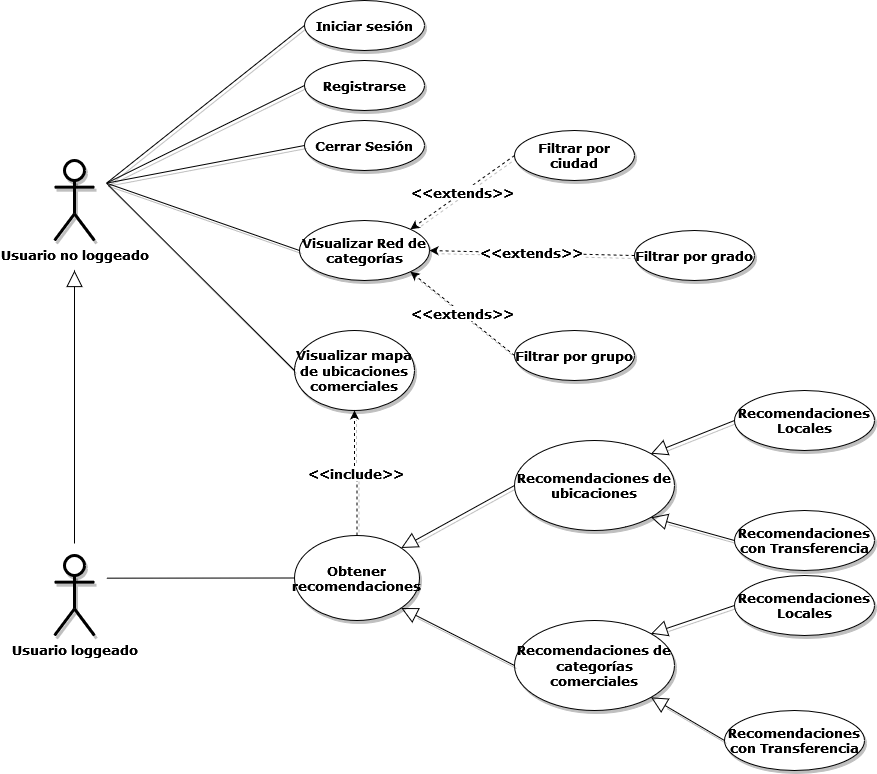
\includegraphics[height=1\textheight]{CasosDeUso}
	\caption{Casos de uso de la aplicación}\label{CasosDeUso}
\end{figure}
\FloatBarrier
%\imagen{CasosDeUso}{Casos de uso de la aplicación}

\end{landscape}


%Una muestra de cómo podría ser una tabla de casos de uso:
%
%% Caso de Uso 1 -> Consultar Experimentos.
%\begin{table}[p]
%	\centering
%	\begin{tabularx}{\linewidth}{ p{0.21\columnwidth} p{0.71\columnwidth} }
	%		\toprule
	%		\textbf{CU-1}    & \textbf{Ejemplo de caso de uso}\\
	%		\toprule
	%		\textbf{Versión}              & 1.0    \\
	%		\textbf{Autor}                & Alumno \\
	%		\textbf{Requisitos asociados} & RF-xx, RF-xx \\
	%		\textbf{Descripción}          & La descripción del CU \\
	%		\textbf{Precondición}         & Precondiciones (podría haber más de una) \\
	%		\textbf{Acciones}             &
	%		\begin{enumerate}
		%			\def\labelenumi{\arabic{enumi}.}
		%			\tightlist
		%			\item Pasos del CU
		%			\item Pasos del CU (añadir tantos como sean necesarios)
		%		\end{enumerate}\\
	%		\textbf{Postcondición}        & Postcondiciones (podría haber más de una) \\
	%		\textbf{Excepciones}          & Excepciones \\
	%		\textbf{Importancia}          & Alta o Media o Baja... \\
	%		\bottomrule
	%	\end{tabularx}
%	\caption{CU-1 Nombre del caso de uso.}
%\end{table}



\begin{table}[p]
	\centering
	\begin{tabularx}{\linewidth}{ p{0.21\columnwidth} p{0.71\columnwidth} }
			\toprule
			\textbf{CU-1}    & \textbf{Iniciar sesión}\\
			\toprule
			\textbf{Versión}              & 1.0    \\
			\textbf{Autor}                & Mario Hurtado \\
			\textbf{Requisitos asociados} & RF-7, RF-7.2, RF-1 \\
			\textbf{Descripción}          & Este caso de uso permite al usuario iniciar sesión con la cuenta con la que se había registrado. \\
			\textbf{Precondición}         & Contar con una cuenta ya registrada en la aplicación.\\
			\textbf{Acciones}             &
			\begin{enumerate}
					\def\labelenumi{\arabic{enumi}.}
					\tightlist
					\item Acceder a la página de inicio de sesión.
					\item Rellenar campo de nombre de usuario.
					\item Rellenar campo de contraseña.
					\item Pulsar en botón de inicio de sesión.
				\end{enumerate}\\
			\textbf{Postcondición}        & Redirección a la página de inicio con la sesión iniciada\\
			\textbf{Excepciones}          & Si el nombre o usuario no son válidos se muestra un mensaje de error. \\
			\textbf{Importancia}          & Alta\\
			\bottomrule
		\end{tabularx}
	\caption{CU-1 Inicio de sesión.}
\end{table}

%
%
\begin{table}[p]
	\centering
	\begin{tabularx}{\linewidth}{ p{0.21\columnwidth} p{0.71\columnwidth} }
			\toprule
			\textbf{CU-2}    & \textbf{Registro de usuario}\\
			\toprule
			\textbf{Versión}              & 1.0    \\
			\textbf{Autor}                & Mario Hurtado \\
			\textbf{Requisitos asociados} & RF-7, RF-7.1, RF-1 \\
			\textbf{Descripción}          & Este caso de uso permite al usuario registrar una cuenta en la aplicación. \\
			\textbf{Precondición}         & Acceder a la página de registro.\\
			\textbf{Acciones}             &
			\begin{enumerate}
					\def\labelenumi{\arabic{enumi}.}
					\tightlist
					\item Rellenar campo de nombre de usuario.
					\item Rellenar campo de nombre.
					\item Rellenar campo de apellido.
					\item Rellenar campo de correo electrónico.
					\item Rellenar campo de contraseña.
					\item Rellenar campo de repetir contraseña
				\end{enumerate}\\
			\textbf{Postcondición}        & \begin{itemize}
				\item Redirección a página de inicio.
				\item Sesión iniciada.
				\item Cuenta registrada en la base de datos.
			\end{itemize} \\
			\textbf{Excepciones}          & Mensaje de error en caso de que uno de los campos no sea válido o el usuario ya exista. \\
			\textbf{Importancia}          & Alta\\
			\bottomrule
		\end{tabularx}
	\caption{CU-2 Registro de usuario.}
\end{table}
%
%%% Caso de Uso 1 -> Consultar Experimentos.
\begin{table}[p]
	\centering
	\begin{tabularx}{\linewidth}{ p{0.21\columnwidth} p{0.71\columnwidth} }
			\toprule
			\textbf{CU-3}    & \textbf{Cierre de sesión}\\
			\toprule
			\textbf{Versión}              & 1.0    \\
			\textbf{Autor}                & Mario Hurtado \\
			\textbf{Requisitos asociados} & RF-7, RF-7.3, RF-1 \\
			\textbf{Descripción}          & Este caso de uso permite al usuario cerrar su sesión. \\
			\textbf{Precondición}         &  Sesión de usuario activa.\\
			\textbf{Acciones}             &
			\begin{enumerate}
					\def\labelenumi{\arabic{enumi}.}
					\tightlist
					\item Pulsar sobre el botón de cierre de sesión
				\end{enumerate}\\
			\textbf{Postcondición}        &  \begin{itemize}
				\item Sesión de usuario cerrada.
				\item Redirección a página de inicio.
			\end{itemize} \\
			\textbf{Excepciones}          & - \\
			\textbf{Importancia}          & Alta \\
			\bottomrule
		\end{tabularx}
	\caption{CU-3 Cierre de sesión de usuario.}
\end{table}
%
%%% Caso de Uso 1 -> Consultar Experimentos.
\begin{table}[p]
	\centering
	\begin{tabularx}{\linewidth}{ p{0.21\columnwidth} p{0.71\columnwidth} }
			\toprule
			\textbf{CU-4}    & \textbf{Visualizar red de categorías.}\\
			\toprule
			\textbf{Versión}              & 1.0    \\
			\textbf{Autor}                & Mario Hurtado \\
			\textbf{Requisitos asociados} & RF-6, RF-6.1, RF-6.3, RF-1 \\
			\textbf{Descripción}          & Este caso de uso permite al usuario visualizar una red de interacción entre categorías. \\
			\textbf{Precondición}         &  - \\
			\textbf{Acciones}             &
			\begin{enumerate}
					\def\labelenumi{\arabic{enumi}.}
					\tightlist
					\item Pulsar en el botón de visualización de red.
				\end{enumerate}\\
			\textbf{Postcondición}        & Redirección a la página de visualización de red de categorías.\\
			\textbf{Excepciones}          &  - \\
			\textbf{Importancia}          & Media \\
			\textbf{Puntos de ampliación} & CU-5, CU-6, CU-7\\
			
			\bottomrule
		\end{tabularx}
	\caption{CU-4 Visualizar red de categorías.}
\end{table}
%
%%% Caso de Uso 1 -> Consultar Experimentos.
\begin{table}[p]
	\centering
	\begin{tabularx}{\linewidth}{ p{0.21\columnwidth} p{0.71\columnwidth} }
			\toprule
			\textbf{CU-5}    & \textbf{Filtro por ciudad en visualización de red}\\
			\toprule
			\textbf{Versión}              & 1.0    \\
			\textbf{Autor}                & Mario Hurtado \\
			\textbf{Requisitos asociados} & RF-6, RF-6.1, RF-6.2, RF-1 \\
			\textbf{Descripción}          & Este caso de uso permite seleccionar de qué ciudad visualizar la red de categorías \\
			\textbf{Precondición}         & Encontrarse en la página de visualización de red\\
			\textbf{Acciones}             &
			\begin{enumerate}
					\def\labelenumi{\arabic{enumi}.}
					\tightlist
					\item El usuario abre el desplegable de ciudades y selecciona una
					\item El sistema hace una petición a la base de datos con la información de las categorías de la ciudad.
					\item La página visualiza la red de categorías.
				\end{enumerate}\\
			\textbf{Postcondición}        & Visualización de la red de categorías de la ciudad seleccionada \\
			\textbf{Excepciones}          & - \\
			\textbf{Importancia}          & Media \\
			\bottomrule
		\end{tabularx}
	\caption{CU-5 Filtro por ciudad en visualización de red.}
\end{table}
%
%%% Caso de Uso 1 -> Consultar Experimentos.
\begin{table}[p]
	\centering
	\begin{tabularx}{\linewidth}{ p{0.21\columnwidth} p{0.71\columnwidth} }
			\toprule
			\textbf{CU-6}    & \textbf{Filtro por grado en visualización de red}\\
			\toprule
			\textbf{Versión}              & 1.0    \\
			\textbf{Autor}                & Mario Hurtado \\
			\textbf{Requisitos asociados} & RF-6, RF-6.4, RF-1 \\
			\textbf{Descripción}          & Este caso de uso permite al usuario aplicar un filtro en base al grado de los nodos en la visualización de la red \\
			\textbf{Precondición}         & Ciudad seleccionada.\\
			\textbf{Acciones}             &
			\begin{enumerate}
					\def\labelenumi{\arabic{enumi}.}
					\tightlist
					\item El usuario selecciona un valor de grado.
					\item El sistema crea un subconjunto de nodos con aquellos con grado mayor o igual al seleccionado.
					\item El sistema actualiza la visualización de red.
				\end{enumerate}\\
			\textbf{Postcondición}        & Visualización de red actualizada con el filtro de grado.\\
			\textbf{Excepciones}          & - \\
			\textbf{Importancia}          & Media \\
			\bottomrule
		\end{tabularx}
	\caption{CU-6 Filtro por grado en visualización de red.}
\end{table}
%
%%% Caso de Uso 1 -> Consultar Experimentos.
\begin{table}[p]
	\centering
	\begin{tabularx}{\linewidth}{ p{0.21\columnwidth} p{0.71\columnwidth} }
			\toprule
			\textbf{CU-7}    & \textbf{Filtro por categoría en visualización de red}\\
			\toprule
			\textbf{Versión}              & 1.0    \\
			\textbf{Autor}                & Mario Hurtado \\
			\textbf{Requisitos asociados} & RF-6, RF-6.5, RF-1 \\
			\textbf{Descripción}          & Este caso de uso permite al usuario filtrar en base a la categoría de los nodos de la visualización de red\\
			\textbf{Precondición}         & Ciudad seleccionada en la visualización de red\\
			\textbf{Acciones}             &
			\begin{enumerate}
					\def\labelenumi{\arabic{enumi}.}
					\tightlist
					\item El usuario selecciona los categoría que desea ver.
					\item El sistema crea un subconjunto con los nodos que se encuentran dentro de las categorías seleccionadas por el usuario.
					\item El sistema reinicia el valor del filtro de grado.
					\item El sistema actualiza la visualización de la red.
				\end{enumerate}\\
			\textbf{Postcondición}        & Visualización de la red actualizada con el filtro de categoría\\
			\textbf{Excepciones}          & - \\
			\textbf{Importancia}          & Media \\
			\bottomrule
		\end{tabularx}
	\caption{CU-7 Filtro por categoría en visualización de red.}
\end{table}

%% Caso de Uso 1 -> Consultar Experimentos.
\begin{table}[p]
	\centering
	\begin{tabularx}{\linewidth}{ p{0.21\columnwidth} p{0.71\columnwidth} }
			\toprule
			\textbf{CU-8}    & \textbf{Visualizar mapa de ubicaciones comerciales}\\
			\toprule
			\textbf{Versión}              & 1.0    \\
			\textbf{Autor}                & Mario Hurtado \\
			\textbf{Requisitos asociados} & RF-3, RF-3.1, RF-3.6, RF-2, RF-1 \\
			\textbf{Descripción}          & Este caso de uso permite a los usuarios visualizar los establecimientos comerciales de distintas categorías en distintas ciudades \\
			\textbf{Precondición}         & -\\
			\textbf{Acciones}             &
			\begin{enumerate}
					\def\labelenumi{\arabic{enumi}.}
					\tightlist
					\item El usuario selecciona una ciudad.
					\item El sistema carga en el menú las categorías comerciales disponibles para la ciudad seleccionada.
					\item El usuario selecciona una categoría comercial.
					\item El sistema sitúa el mapa en las coordenadas de la ciudad.
					\item El sistema muestra los marcadores con los establecimientos comerciales en el mapa
				\end{enumerate}\\
			\textbf{Postcondición}        & Mapa situado en las coordenadas de la ciudad seleccionada y con los marcadores correspondientes a la categoría elegida.\\
			\textbf{Excepciones}          & - \\
			\textbf{Importancia}          & Alta \\
			\bottomrule
		\end{tabularx}
	\caption{CU-8 Visualizar mapa de ubicaciones comerciales.}
\end{table}

%% Caso de Uso 1 -> Consultar Experimentos.
\begin{table}[p]
	\centering
	\begin{tabularx}{\linewidth}{ p{0.21\columnwidth} p{0.71\columnwidth} }
			\toprule
			\textbf{CU-9}    & \textbf{Recomendaciones de ubicaciones a nivel local}\\
			\toprule
			\textbf{Versión}              & 1.0    \\
			\textbf{Autor}                & Mario Hurtado \\
			\textbf{Requisitos asociados} & RF-3, RF-3.2, RF3.4, RF-3.5, RF-3.6, RF-3.7, RF-3.8, RF-5, RF-5.1, RF-1  \\
			\textbf{Descripción}          & Este caso de uso permite al usuario obtener recomendaciones a nivel local en base a ubicaciones que haya seleccionado\\
			\textbf{Precondición}         & \begin{itemize}
							\tightlist
				\item Usuario con sesión iniciada.
				\item Encontrarse en la página del mapa.
				\end{itemize}\\
			\textbf{Acciones}             &
			\begin{enumerate}
					\def\labelenumi{\arabic{enumi}.}
					\tightlist
					\item El usuario selecciona los establecimientos y ubicaciones en los que está interesado
					\item El usuario pulsa el botón de recomendaciones de ubicaciones a nivel local.
					\item El sistema redirige a la página de recomendaciones a nivel local, mostrando en el mapa las ubicaciones seleccionadas con un identificador.
					\item El sistema calcula los valores para las recomendaciones.
					\item El usuario selecciona la categoría comercial en la que está interesado.
					\item El usuario selecciona el método a emplear.
					\item El sistema muestra las ubicaciones seleccionadas ordenadas en orden descendente según la adecuación a la categoría seleccionada.
				\end{enumerate}\\
			\textbf{Postcondición}        & Resultados de recomendaciones de ubicaciones. Orden descendente según adecuación a la categoría seleccionada\\
			\textbf{Incluye}   & CU-8\\
			\textbf{Excepciones}          & - \\
			\textbf{Importancia}          & Alta  \\
			\bottomrule
		\end{tabularx}
	\caption{CU-9 Recomendaciones de ubicaciones a nivel local.}
\end{table}

\begin{table}[p]
	\centering
	\begin{tabularx}{\linewidth}{ p{0.21\columnwidth} p{0.71\columnwidth} }
		\toprule
		\textbf{CU-10}    & \textbf{Recomendaciones de ubicaciones con transferencia}\\
		\toprule
		\textbf{Versión}              & 1.0    \\
		\textbf{Autor}                & Mario Hurtado \\
		\textbf{Requisitos asociados} & RF-3, RF-3.2, RF3.4, RF-3.5, RF-3.6, RF-3.7, RF-3.8, RF-5, RF-5.2, RF-1  \\
		\textbf{Descripción}          & Este caso de uso permite al usuario obtener recomendaciones en base a ubicaciones que haya seleccionado empleando transferencia de conocimiento.\\
		\textbf{Precondición}         & \begin{itemize}
						\tightlist
			\item Usuario con sesión iniciada.
			\item Encontrarse en la página del mapa.
		\end{itemize}\\
		\textbf{Acciones}             &
		\begin{enumerate}
			\def\labelenumi{\arabic{enumi}.}
			\tightlist
			\item El usuario selecciona los establecimientos y ubicaciones en los que está interesado
			\item El usuario pulsa el botón de recomendaciones de ubicaciones con transferencia.
			\item El sistema redirige a la página de recomendaciones con transferencia, mostrando en el mapa las ubicaciones seleccionadas con un identificador.
			\item El usuario selecciona una ciudad.
			\item El sistema actualiza las categorías disponibles
			\item El sistema calcula los valores para las recomendaciones.
			\item El usuario selecciona la categoría comercial en la que está interesado.
			\item El usuario selecciona el método a emplear.
			\item El sistema muestra las ubicaciones seleccionadas ordenadas en orden descendente según la adecuación a la categoría seleccionada.
		\end{enumerate}\\
		\textbf{Postcondición}        & Resultados de recomendaciones de ubicaciones. Orden descendente según adecuación a la categoría seleccionada\\
		\textbf{Incluye}   & CU-8\\
		\textbf{Excepciones}          & - \\
		\textbf{Importancia}          & Alta  \\
		\bottomrule
	\end{tabularx}
	\caption{CU-10 Recomendaciones de ubicaciones con transferencia.}
\end{table}

\begin{table}[p]
	\centering
	\begin{tabularx}{\linewidth}{ p{0.21\columnwidth} p{0.71\columnwidth} }
		\toprule
		\textbf{CU-11}    & \textbf{Recomendaciones de categorías a nivel local}\\
		\toprule
		\textbf{Versión}              & 1.0    \\
		\textbf{Autor}                & Mario Hurtado \\
		\textbf{Requisitos asociados} & RF-3, RF-3.2, RF3.4, RF-3.5, RF-3.6, RF-3.7, RF-3.8, RF-4, RF-4.1, RF-1  \\
		\textbf{Descripción}          & Este caso de uso permite al usuario obtener recomendaciones de categorías en base a las ubicaciones que haya seleccionado a nivel local.\\
		\textbf{Precondición}         & \begin{itemize}
						\tightlist
			\item Usuario con sesión iniciada.
			\item Encontrarse en la página del mapa.
		\end{itemize}\\
		\textbf{Acciones}             &
		\begin{enumerate}
			\def\labelenumi{\arabic{enumi}.}
			\tightlist
			\item El usuario selecciona los establecimientos y ubicaciones en los que está interesado
			\item El usuario pulsa el botón de recomendaciones de categorías a nivel local.
			\item El sistema redirige a la página de recomendaciones de categorías a nivel local, mostrando en el mapa las ubicaciones seleccionadas con un identificador.
			\item El sistema calcula los valores para las recomendaciones.
			\item El usuario selecciona el método a emplear.
			\item El sistema muestra las ubicaciones seleccionadas junto con las categorías comerciales más adecuadas para cada una.
		\end{enumerate}\\
		\textbf{Postcondición}        & Resultados de recomendaciones de categorías para cada ubicación\\
		\textbf{Incluye}   & CU-8\\
		\textbf{Excepciones}          & - \\
		\textbf{Importancia}          & Alta  \\
		\bottomrule
	\end{tabularx}
	\caption{CU-11 Recomendaciones de categorías a nivel local.}
\end{table}


\begin{table}[p]
	\centering
	\begin{tabularx}{\linewidth}{ p{0.21\columnwidth} p{0.71\columnwidth} }
		\toprule
		\textbf{CU-12}    & \textbf{Recomendaciones de categorías con transferencia}\\
		\toprule
		\textbf{Versión}              & 1.0    \\
		\textbf{Autor}                & Mario Hurtado \\
		\textbf{Requisitos asociados} & RF-3, RF-3.2, RF3.4, RF-3.5, RF-3.6, RF-3.7, RF-3.8, RF-4, RF-4.2, RF-1  \\
		\textbf{Descripción}          & Este caso de uso permite al usuario obtener recomendaciones de categorías en base a las ubicaciones que haya seleccionado empleando transferencia.\\
		\textbf{Precondición}         & \begin{itemize}
			\tightlist
			\item Usuario con sesión iniciada.
			\item Encontrarse en la página del mapa.
		\end{itemize}\\
		\textbf{Acciones}             &
		\begin{enumerate}
			\def\labelenumi{\arabic{enumi}.}
			\tightlist
			\item El usuario selecciona los establecimientos y ubicaciones en los que está interesado
			\item El usuario pulsa el botón de recomendaciones de categorías con transferencia.
			\item El sistema redirige a la página de recomendaciones de categorías con transferencia, mostrando en el mapa las ubicaciones seleccionadas con un identificador.
			\item El usuario selecciona una ciudad.
			\item El sistema calcula las recomendaciones.
			\item El usuario selecciona el método a emplear.
			\item El sistema muestra las ubicaciones seleccionadas junto con las categorías comerciales más adecuadas para cada una.
		\end{enumerate}\\
		\textbf{Postcondición}        & Resultados de recomendaciones de categorías para cada ubicación según la ciudad seleccionada.\\
		\textbf{Incluye}   & CU-8\\
		\textbf{Excepciones}          & - \\
		\textbf{Importancia}          & Alta  \\
		\bottomrule
	\end{tabularx}
	\caption{CU-12 Recomendaciones de categorías con transferencia.}
\end{table}
\apendice{Especificación de diseño}

\section{Introducción}

En esta sección se explicará la estructura de los datos de la aplicación, así como de su arquitectura y su funcionamiento.

\section{Diseño de datos}
Un aspecto a tener en consideración en cuanto a la estructura de los datos es que no estamos utilizando una base de datos relacional, y por tanto no contamos con una estructura de tablas. Neo4j es una base de datos NoSQL orientada a grafos, por tanto la 2 entidades con la que estructurar la base de datos son los nodos y enlaces. Ambas entidades cuentan con etiquetas propias para poder identificar su tipo. Explicaré todas aquellas utilizadas en este trabajo.

\subsection{Nodos}

En cuanto a nodos de la base de datos contamos con principales etiquetas \texttt{:Place} para los lugares y \texttt{:Category} para las categorías.

\subsubsection{\texttt{:Place}}

Los nodos con esta etiqueta son cada una de las ubicaciones obtenidas de OpenStreetMap. Cuenta con los siguientes atributos:

\begin{itemize}
	\item \texttt{area}: \textit{String} con el nombre de la ciudad a la que pertenecen.
	\item \texttt{category}: \textit{String} con el nombre de la categoría comercial a la que pertenece,
	\item \texttt{coords}: Tipo \textit{Point} de Neo4j con las coordenadas de la ubicación.
	\item \texttt{id}: \textit{Integer} con el número identificativo de la ubicación en OpenStreetMap
	\item \texttt{type}: \textit{String} identificativo de si la categoría de este nodo pertenece a \textit{amenity} o \textit{shop}.
	\item \texttt{Q}: JSON serializado en formato \textit{String} que contiene los índices de calidad para dicha ubicación.
\end{itemize}

Los campos anteriores son los que están presentes en todos los nodos de este tipo. Algunos nodos contienen atributos adicionales con la información que OpenStreetMap provee para dicha ubicación, estos pueden ser nombre, teléfono, página web, entre otros.

\subsubsection{\texttt{:Category}}
Estos nodos son los constitutivos de la red de categorías de cada ciudad. Cada una estará compuesta por las categorías presentes únicamente en esa ciudad.

Cada nodo posee los siguientes atributos:

\begin{itemize}
	\item \texttt{city}: \textit{String} con la ciudad a la que pertenece dicha categoría.
	\item \texttt{n\_nodes}: \textit{Integer} con el número de nodos que posee dicha categoría en esa ciudad.
	\item \texttt{name}: \textit{String} con el nombre de la categoría comercial.
	\item \texttt{type}: \textit{String} con el tipo de categoría entre \textit{amenity} y \textit{shop}
\end{itemize}

\subsubsection{\texttt{:User}}
Si bien los usuarios no juegan un papel importante en comparación a las otras entidades estos también deben de contar con una representación en la base de datos.

Cuentan con los siguientes atributos:

\begin{itemize}
	\item \texttt{userId}: \textit{String} con UUID identificativo del usuario.
	\item \texttt{user\_name}: \textit{String} con el nombre de usuario.
	\item \texttt{password}: \textit{String} con la contraseña cifrada del usuario.
	\item \texttt{name}: \textit{String} con el nombre personal del usuario.
	\item \texttt{surname}: \textit{String} con el apellido del usuario.
	\item \texttt{role}: \textit{String} con el rol del usuario.
	\item \texttt{mail}: \textit{String} con correo electrónico del usuario.
\end{itemize}

\subsection{Enlaces}
La otra entidad con la que contamos en la base de datos son los enlaces. Estos más allá de servir como simple enlace entre nodos, también pueden almacenar atributos además de poder asignarles etiquetas identificativas.

\subsubsection{\texttt{:IS\_NEAR}}
Este tipo de enlaces son aquellos representativos de la proximidad entre ubicaciones comerciales. Al igual que se indicaba en la memoria, estos se crean únicamente entre nodos con una distancia entre sí menor o igual a 100 metros.

Cuentan con un único atributo de nombre \texttt{distance} de tipo \textit{Float} con la distancia entre los dos nodos enlazados.

Este tipo de enlace solo une nodos etiquetados como \texttt{:Place}.

\subsubsection{\texttt{:Rel}}
Estos enlaces son representativos de las interacciones entre categorías. Dado que necesitamos contar con la matriz de interacción, la red de categorías tendrá un subgrafo compuesto por los nodos categoría de una ciudad y con enlaces de este tipo conectando cada par de estos nodos.

Cada uno de estos enlaces tiene los siguientes atributos:
\begin{itemize}
	\item \texttt{real\_value}: \textit{Integer} con el valor real de interacción entre el par de categorías.
	\item \texttt{a\_ij}: \textit{Float} con el valor de la matriz de coeficientes del método \textit{Permutation}.
	\item \texttt{perc\_25}: \textit{Float} con el valor del percentil 0.25 de las simulaciones.
	\item \texttt{perc\_975}: \textit{Float} con el valor del percentil 0.975 de las simulaciones.
	\item \texttt{std\_dev}: \textit{Float} con el valor de la desviación estandar de las simulaciones.
	\item \texttt{mean}: \textit{Float} con el valor de la media de las simulaciones.
	\item \texttt{z-score}: \textit{Float} con el \textit{Z-Score} de las simulaciones.
	\item \texttt{relevant}: \textit{Bool} indicando si la relación entre categorías se encuentra entre las estadísticamente relevantes
\end{itemize}

\subsubsection{\texttt{:Jensen}}
Estas relaciones representan la matriz de coeficientes de Jensen. Un característica a tener en cuenta de esto es que la matriz no es simétrica, esto implica que entre cada par de nodos de categorías por ciudad existan 2 enlaces dirigidos entre ellas.

Estos enlaces solo cuentan con un único atributo de nombre \texttt{coeff}, de tipo \textit{Float} con el valor del coeficiente de Jensen para una categoría sobre otra.

\section{Diseño procedimental}

\newpage
\subsection{Inicio de sesión}
\begin{figure}[!h]
	\centering
	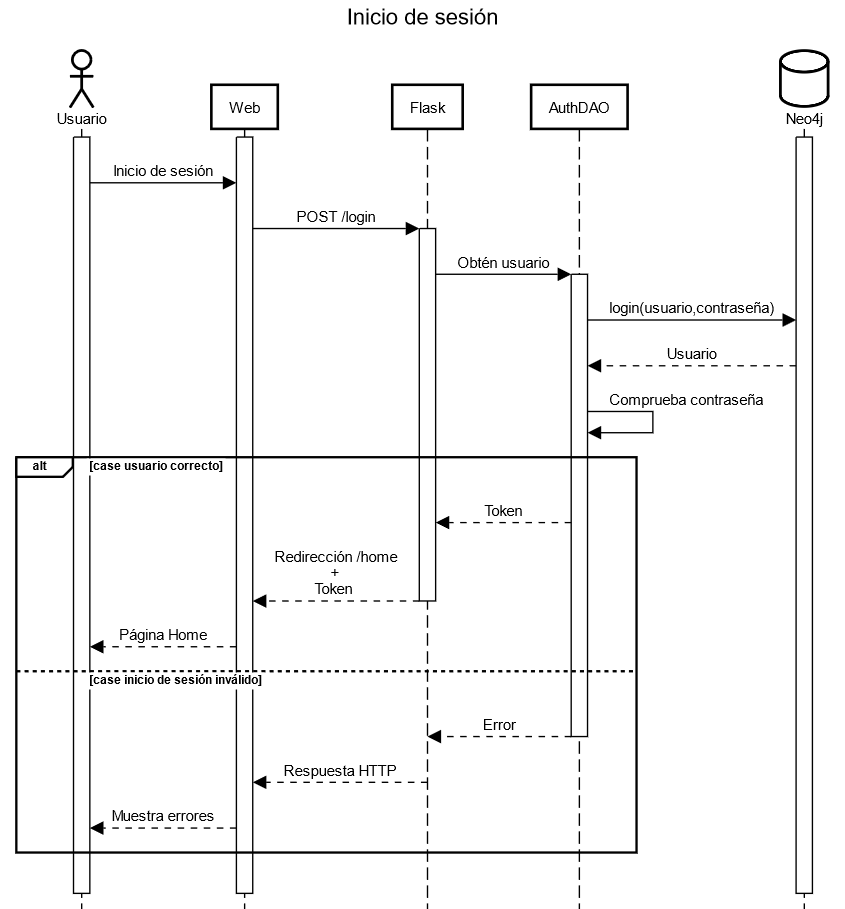
\includegraphics[height=0.8\textheight]{LoginSeq}
	\caption{Diagrama de secuencia de inicio de sesión}\label{LoginSeq}
\end{figure}
\FloatBarrier

\newpage

\subsection{Registro}

	\begin{figure}[!h]
		\centering
		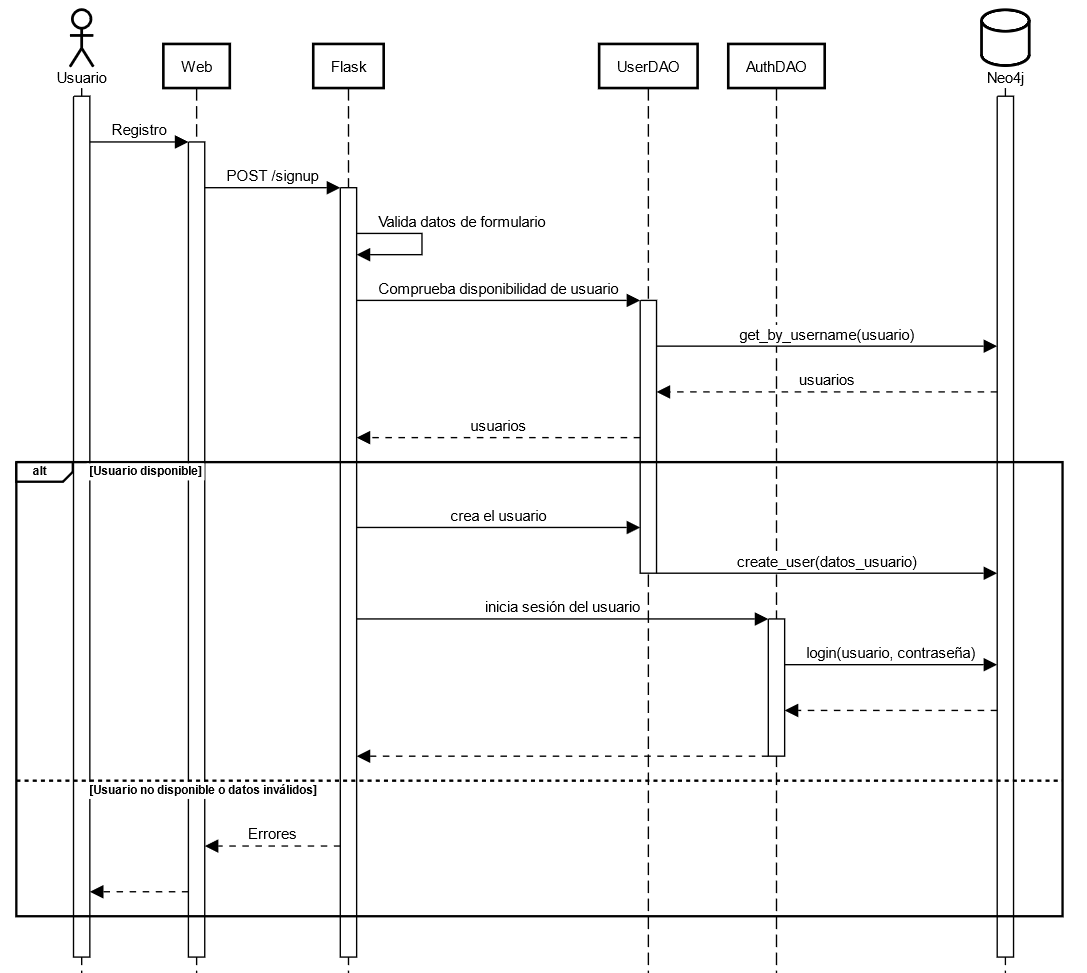
\includegraphics[width=1\textwidth]{SignUpSeq}
		\caption{Diagrama de secuencia de registro}\label{SignUpSeq}
	\end{figure}
	\FloatBarrier

\newpage



\begin{landscape}
	\subsection{Selección de ciudad}
	\begin{figure}[!h]
		\centering
		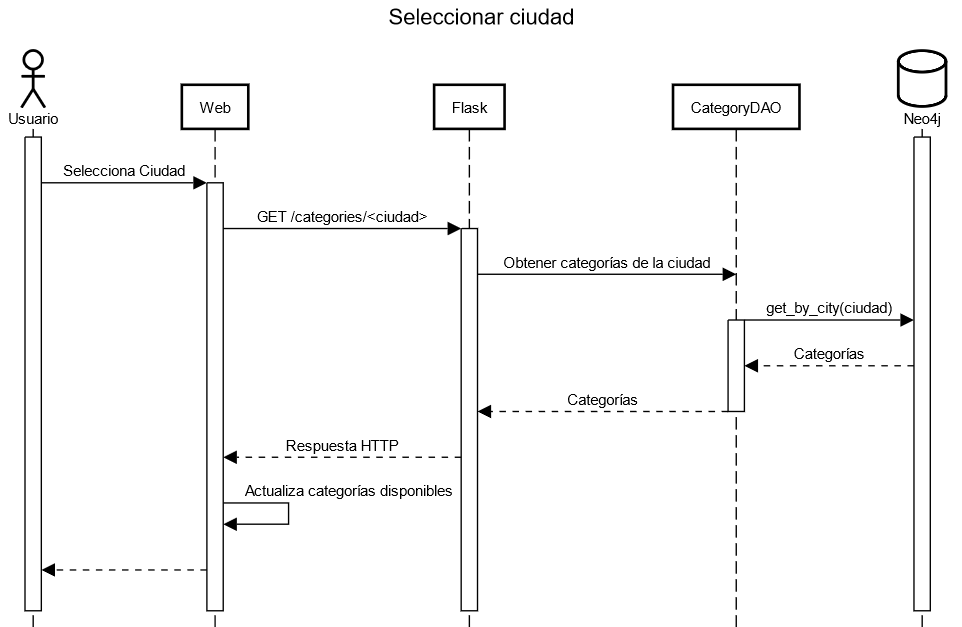
\includegraphics[height=0.8\textheight]{CityCats}
		\caption{Diagrama de secuencia de selección de ciudad}\label{CityCats}
	\end{figure}
	\FloatBarrier
\end{landscape}

\subsection{Recomendaciones de categorías}
	\begin{figure}[!h]
	\centering
	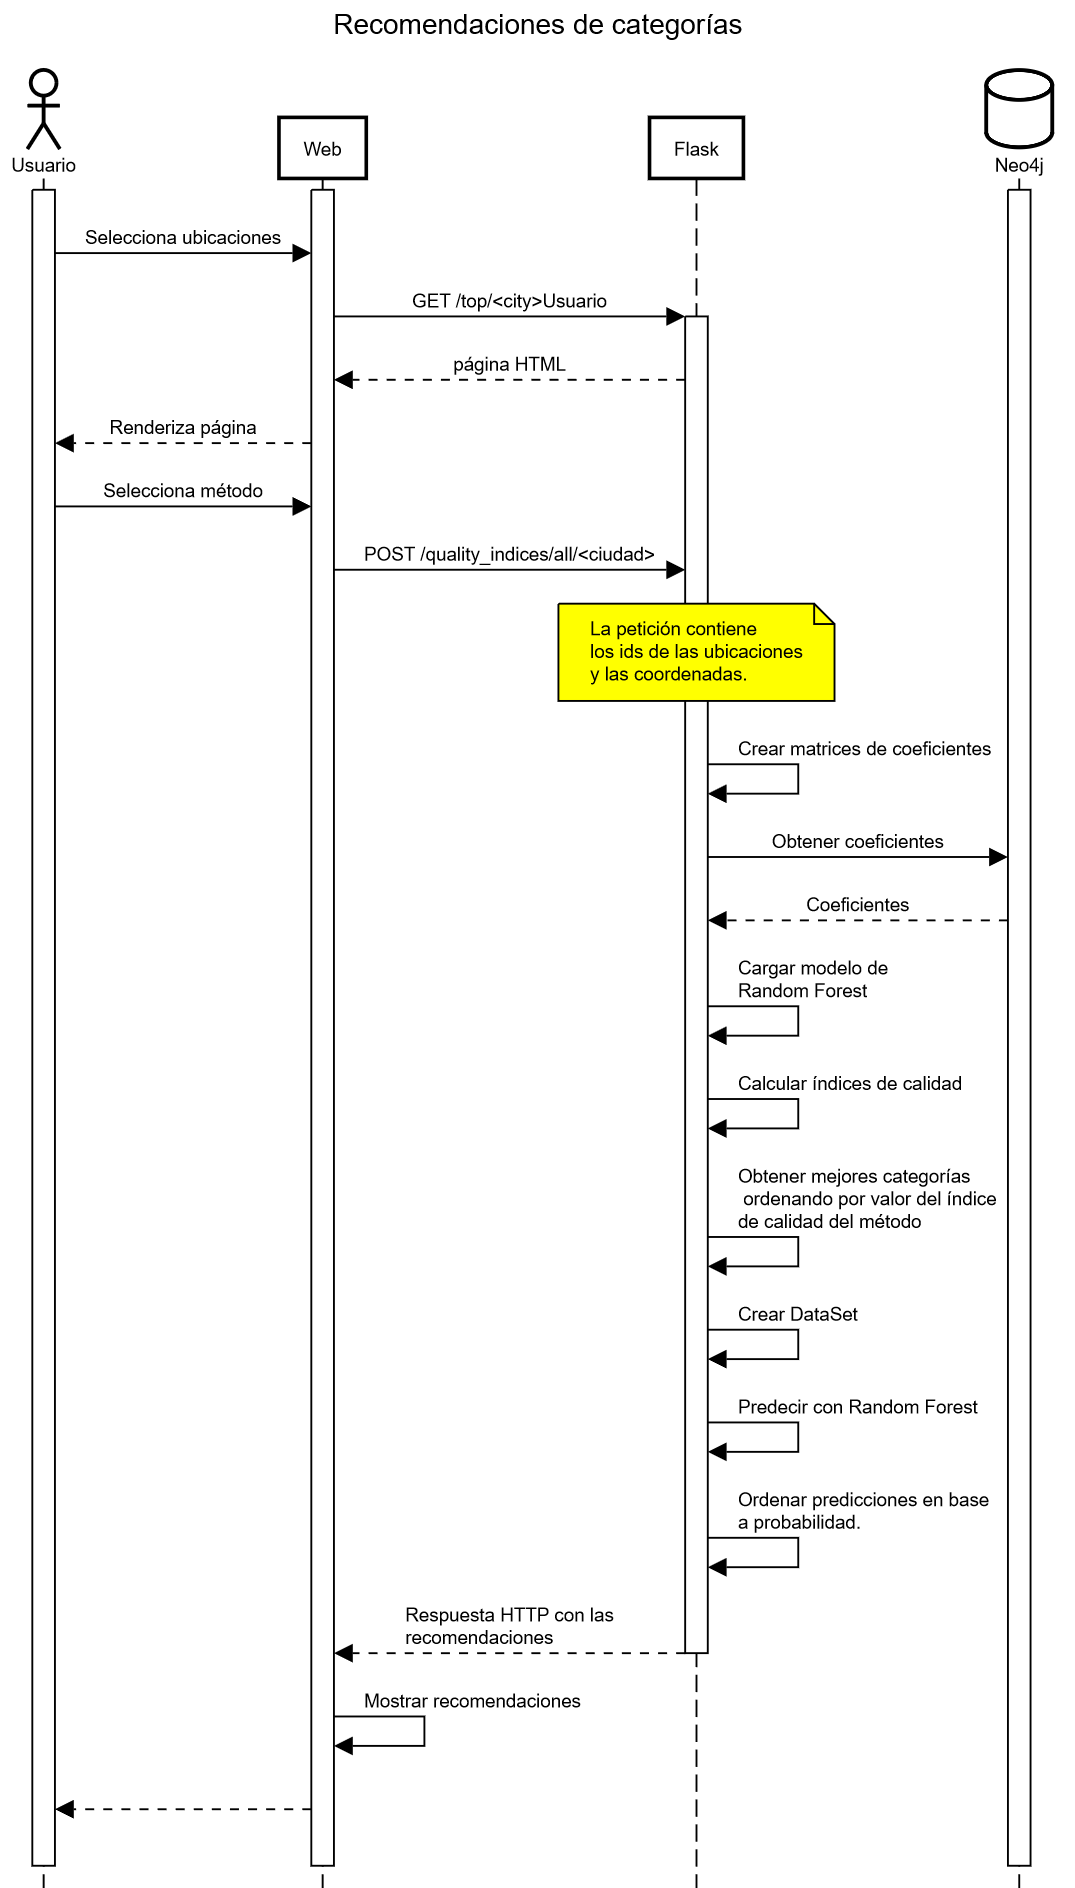
\includegraphics[height=0.8\textheight]{TopsCatsSeq}
	\caption{Diagrama de secuencia de obtención de recomendaciones de categorías}\label{TopsCatsSeq}
\end{figure}
\FloatBarrier
\newpage
\subsection{Recomendaciones de ubicaciones}
	\begin{figure}[!h]
	\centering
	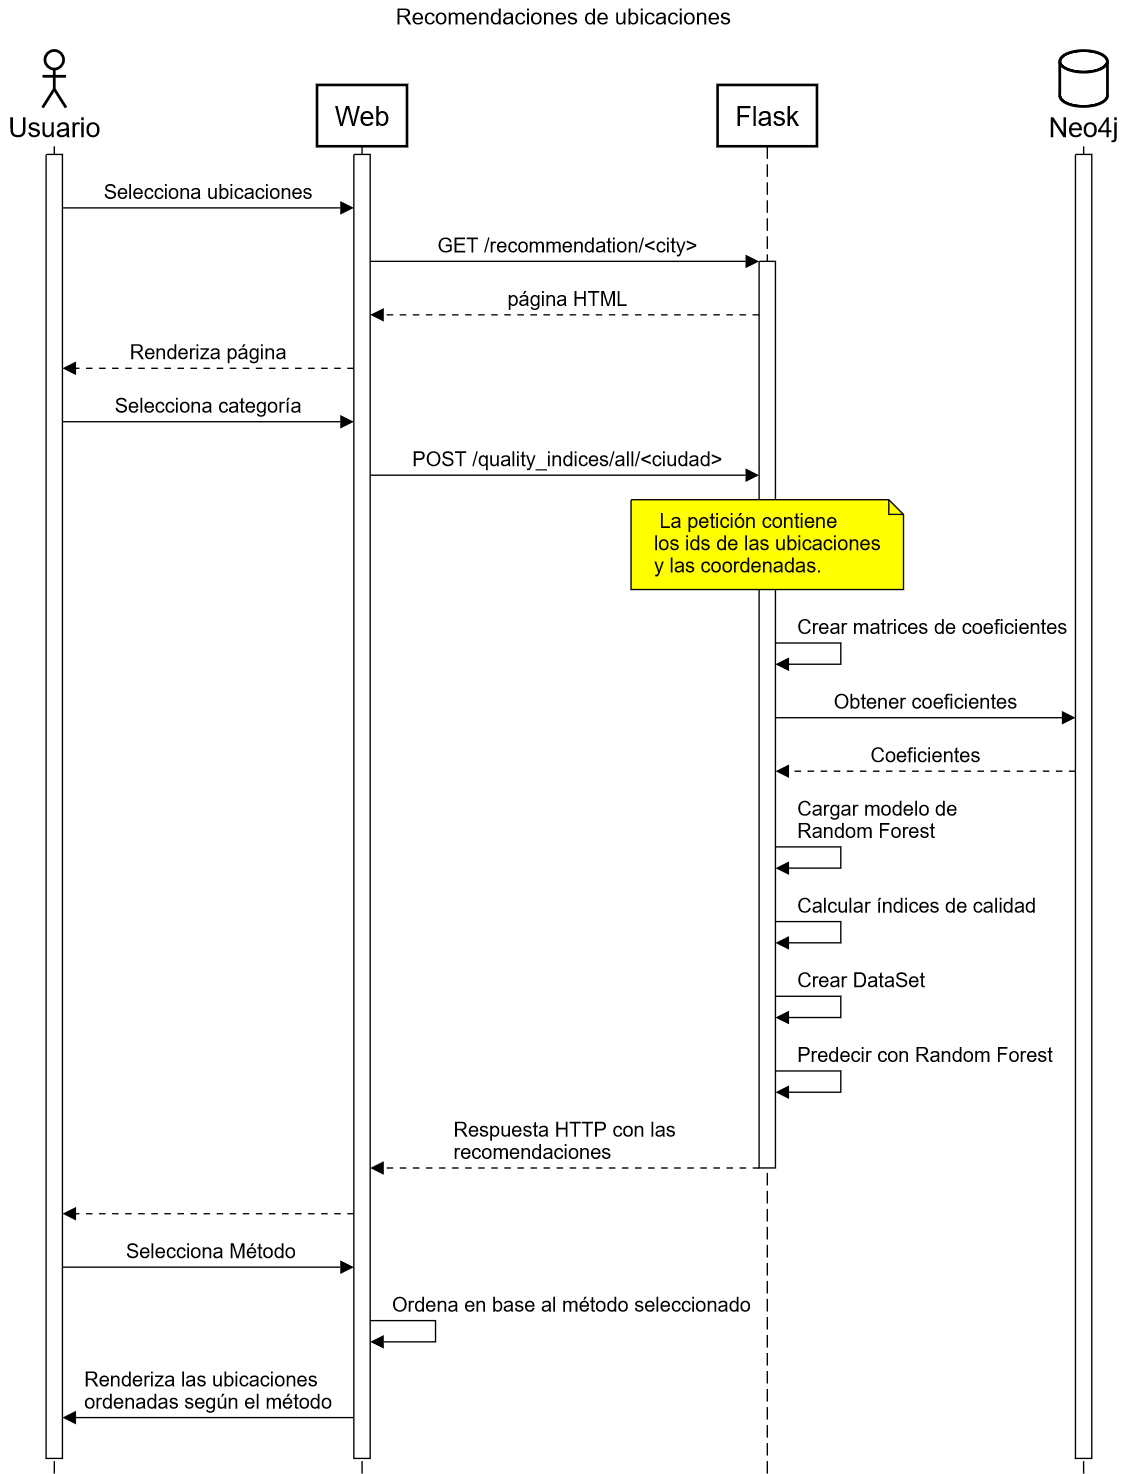
\includegraphics[height=0.8\textheight]{TopsPlacesSeq}
	\caption{Diagrama de secuencia de obtención de recomendaciones de ubicaciones}\label{TopsPlacesSeq}
\end{figure}
\FloatBarrier

\newpage
\subsection{Visualización de red de categorías}
	\begin{figure}[!h]
	\centering
	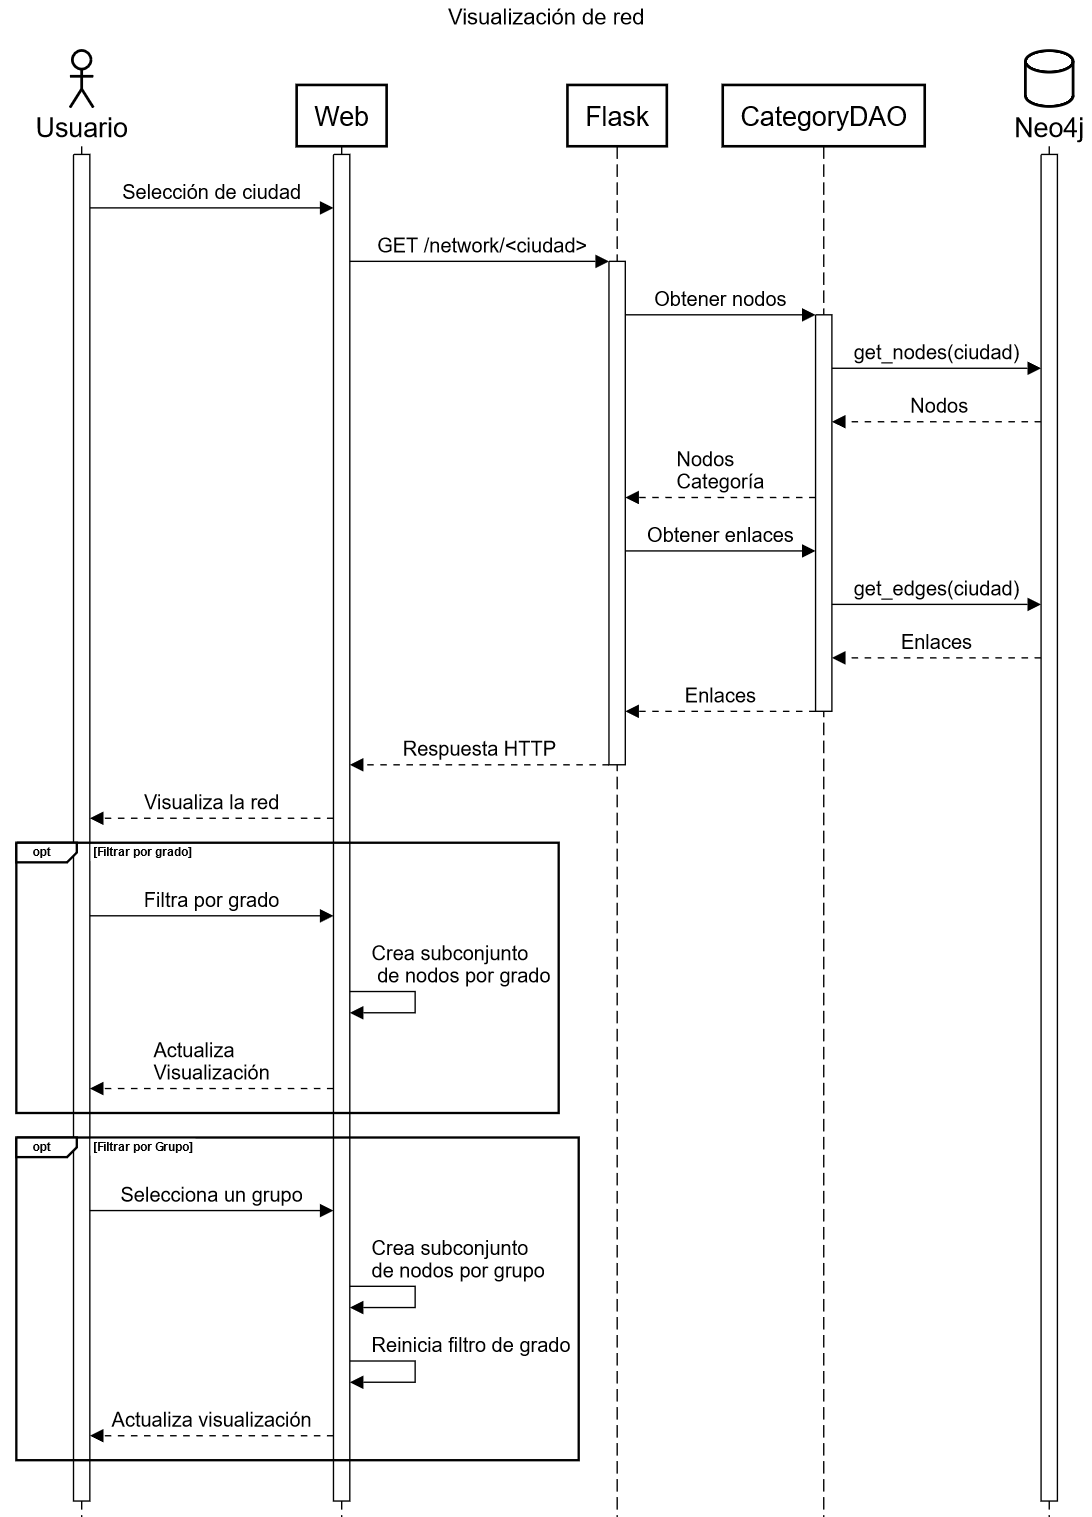
\includegraphics[height=0.8\textheight]{NetworkSeq}
	\caption{Diagrama de secuencia de visualización de red de categorías}\label{NetworkSeq}
\end{figure}
\FloatBarrier
\newpage

\section{Diseño arquitectónico}

Dado que el producto final de este trabajo es una aplicación web conviene mencionar unas estructuras propias de este tipo de aplicaciones.

\subsection{Arquitectura Cliente-Servidor}
La arquitectura cliente servidor es un modelo ampliamente utilizado en el entorno web. Esta está compuesta por dos entidades distintas con diferentes responsabilidades.

\begin{itemize}
	\item Cliente:
	\begin{itemize}
		\item Realiza peticiones al servidor para obtener los recursos o servicios.
		\item Provee una interfaz gráfica al usuario.
		\item Recibe las respuestas del servidor.
	\end{itemize}
	\item Servidor:
	\begin{itemize}
		\item Responde a las peticiones del cliente.
		\item Se encarga de manejar la lógica de negocio y la gestión de recursos.
		\item Puede contar con una conexión con una base de datos en la que puede almacenar y extraer la información requerida.
	\end{itemize}
\end{itemize}

\imagen{ClienteServidor}{Esquema Cliente-Servidor}

En el contexto web y de nuestro proyecto el cliente es el dispositivo desde el que el usuario accede a la aplicación, haciendo peticiones al servidor web mediante el protocolo HTTP. En cuanto al servidor este será el equipo que alojará la aplicación web.
\subsection{Modelo-Vista-Controlador}

El patrón Modelo-Vista-Controlador o MVC se trata de una arquitectura utilizada ampliamente para estructurar proyectos \textit{software}. Esta define 3 distintos componentes con responsabilidades distintas del funcionamiento del programa. Esto permite tener separada la lógica de la aplicación en componentes en base a la responsabilidad que toma, facilitando la organización y futuro mantenimiento.

\imagen{MVC}{Esquema de arquitectura Modelo-Vista-Controlador}

Las partes que componen MVC son las siguientes:
\begin{itemize}
	\item Modelo: El componente Modelo contiene toda la lógica relacionada a los datos, su estructura y manejo. Normalmente interactúa con una base de datos, que es donde aloja la información de la aplicación.
	\item Vista: Es el componente encargado de presentar una interfaz al usuario donde mostrar la información de la aplicación y poder interactuar con esta.
	\item Controlador: Es el componente intermedio entre en el Modelo y la Vista. Se encarga de dar una respuesta adecuada a las entradas del usuario en la Vista e interactuar con el Modelo para modificar la información de la aplicación según la lógica de esta. 
\end{itemize}

Aplicado a nuestro proyecto el componente Modelo se correspondería a los distintos DAOs contenidos en \texttt{/src/web/dao}.

El controlador está compuesto por las distintas rutas definidas en la aplicación Flask en el directorio \texttt{/src/web/routes} junto con la lógica definida en cada uno de ellos para el tratamiento de las peticiones del usuario.

En cuanto a la vista, esta sería todo aquello que se ejecutaría en el lado del servidor, siendo esto plantillas HTML, hojas de estilo y scripts de JavaScript, todo ello contenido dentro del directorio \texttt{/src/web/static}. Esto se corresponde con los ficheros contenidos dentro de \texttt{/templates}, \texttt{/styles} y \texttt{/js} respectivamente. Estas vistas serían aquellas devueltas por las rutas definidas en \texttt{/src/web/routes/views}.
\apendice{Documentación técnica de programación}

\section{Introducción}
En este apartado se desarrollará sobre la estructura del proyecto así como las partes que lo componen y la función de cada una. El código fuente de este trabajo puede encontrarse en el siguiente \href{https://github.com/mariohu2001/TFG-Urban-Street-Mapping-Transfer}{repositorio de GitHub}.
\section{Estructura de directorios}

El código fuente que compone el proyecto está completamente contenido dentro de la carpeta \texttt{/src}.

\subsection{\texttt{/web}}
Esta carpeta contiene todo el código necesario para el funcionamiento de la aplicación web.

\subsubsection{\texttt{/web/dao}}
Este directorio contiene los conocidos como DAOs (\textit{Data Access Object}). Los ficheros contenidos dentro definen clases que permiten acceder y modificar de una forma cómoda los datos contenidos dentro de Neo4j. En los métodos de cada DAO se utilizan sentencias de Cypher, el lenguaje de consultas de Neo4j para realizar la información que deseamos.

Tiene los siguientes ficheros:
\begin{itemize}
	\item \texttt{baseDAO.py}: Clase base de la que heredan el resto de DAOs.
	\item \texttt{authDAO.py}: DAO encargado de la autenticación de usuarios.
	\item \texttt{categoryDAO.py}: DAO encargado de la obtención y modificación de la información de las categorías.
	\item \texttt{coordsDAO.py}: Este DAO está centrado en la obtención de índices de calidad dadas unas coordenadas. Dada la complejidad de esto último se estimó encapsular la lógica en esta clase.
	\item \texttt{placesDAO.py}: Este fichero contiene el DAO orientado a los lugares almacenados en la base de datos. Posee funciones para listar en base a ciudad o categoría, además de algunas para calcular índices de calidad.
	\item \texttt{usersDAO.py}: En esta clase está contenida la lógica de creación de usuarios así como la obtención de datos de estos.
\end{itemize}

\subsubsection{\texttt{/web/models}}
Este directorio contiene los distintos modelos de \textit{Random Forest} serializados y comprimidos en ficheros individuales para cada uno. Posee dos subdirectorios, \texttt{/local} y \texttt{/transfer}, siendo el primero para los modelos a nivel local y el segundo para los modelos usados para hacer transferencia.

En el caso de \texttt{/local}, los modelos están almacenados siguiente la convención de nombres \texttt{/\textit{Ciudad}.gz}. Esta debe respetarse para poder cargar adecuadamente los ficheros.

En cuanto a \texttt{/transfer}, sigue una convención similar al anterior, siendo esta \texttt{/\textit{CiudadOrigen}-\textit{CiudadDestino}.gz}. Esto debe tenerse en cuenta para cargar los modelos adecuadamente.

\subsubsection{\texttt{/web/routes}}
Este directorio contiene las distintas rutas de la API definidas con \textit{Blueprints} de Flask, estos permiten definir rutas más allá del fichero donde se define la aplicación de Flask. Aquí las rutas están agrupadas en módulos en base al ámbito al que pertenezcan.

Existe un subdirectorio de nombre \texttt{views} que contiene todas aquellas rutas que como respuesta devuelven una plantilla HTML. A su vez estas están agrupadas en los siguientes módulos:

\begin{itemize}
	\item \texttt{/account.py}: Contiene los \textit{endpoints} relacionados a usuarios, inicio de sesión y registro.
	\item \texttt{/common.py}: Este módulo contiene los \textit{endpoints} generales o los que no encajan en ningún otro módulo. En este caso \textit{home} y la visualización de la red de categorías.
	\item \texttt{/maps.py}: Este fichero contiene todos aquellos \textit{endpoints} que contengan una visualización de un mapa en la plantilla devuelta como respuesta.
\end{itemize}

Los siguientes módulos definen \textit{endpoints} que no tienen una plantilla como respuesta. Estos suelen usar los métodos HTTP \textit{GET} y \textit{POST} ; tienen la función de obtener determinados datos del lado del servidor o procesar algunos incluidos en el cuerpo de la petición.

Los \textit{endpoints} están agrupados en 2 módulos:
\begin{itemize}
	\item \texttt{/category.py}: Define rutas con relación a las categorías, pudiendo devolver datos en función de categoría o ciudad.
	\item \texttt{/places.py}: Especifica los \textit{endpoints} relacionados con los lugares almacenados en la base de datos. Estos consisten en la obtención de ubicaciones en base a categoría o ciudad, así como los índices de calidad y recomendaciones de categorías.
\end{itemize}

\subsubsection{\texttt{/web/static}}
Este directorio contiene todo lo relacionado con el procesamiento por parte del navegador, o es decir, del cliente. El nombre es debido a que se trata de una convención para este el directorio que contiene este tipo de ficheros.

Este contiene 4 subdirectorios:
\begin{itemize}
	\item \texttt{/img}: Contiene los archivos de imagen utilizados en la página web.
	\item \texttt{/js}: En este directorio se guardan todos los scripts de JavaScript utilizados en las distintas plantillas HTML.
	\item \texttt{/styles}: Este directorio contiene todos los ficheros con hojas de estilo CSS utilizadas por las plantillas HTML.
	\item \texttt{/templates}: Contiene todos los ficheros HTML utilizados por la aplicación web. A su vez contiene un subdirectorio de nombre \texttt{/macros} donde se encuentran definidas algunas \textit{macros} propias del motor de plantillas Jinja2.
\end{itemize} 

\subsubsection{Otros módulos}
Además de los ficheros contenidos en directorios existen algunos que cuelgan directamente de \texttt{/web}. Estos son los siguientes:

\begin{itemize}
	\item \texttt{\_\_init\_\_.py}: Este ficheros, con un nombre que se suele utilizar para definir módulos en Python, contiene la creación de la aplicación Flask así como su configuración.
	\item \texttt{authentication.py}: Fichero que define un decorador para restringir el acceso a determinados \textit{endpoints} si no se posee un determinado rol.
	\item \texttt{driver\_neo4j.py}: Contiene la inicialización del \textit{driver} de Neo4j para la aplicación web.
	\item \texttt{forms.py}: Contiene la definición de formularios a utilizar en las plantillas usando la librería Flask-WTF.
	\item \texttt{quality\_indices.py}: Módulo que contiene métodos auxiliares para calcular los índices de calidad.
	\item \texttt{utils.py}: Fichero de propósito general que define utilidades varias.
\end{itemize}


\subsection{\texttt{/models}}
En este directorio se encuentran unos ficheros en formato \textit{Jupyter Notebook} utilizados para la creación de los modelos de \textit{Random Forest}. Además se cuenta con el \textit{dataset} requerido para el entrenamiento de los modelos en el subdirectorio \texttt{/models/dataset}. Los ficheros de este están en formato JSON, puesto que es el más adecuado para almacenar estos datos. Cada ciudad cuenta con un fichero.

\subsection{\texttt{/operaciones\_bbdd}}
En este directorio se encuentran todos los \textit{scripts} utilizados para la carga de ubicaciones en la base de datos, así como distintas operaciones de uso más general que no son utilizadas en la aplicación web.

\subsubsection{/\texttt{docker}}
En este directorio se encuentran los \textit{Dockerfile} necesarios para usar Docker en este proyecto.

Contamos con los siguientes ficheros:

\begin{itemize}
	\item \texttt{Dockerfile.neo4j}: Fichero necesario para la construcción de la imagen de Neo4j que se utilizará en el proyecto. Requiere de un fichero \texttt{neo4f.dump} para crear la base de datos cargada con los datos utilizados.
	\item \texttt{Dockerfile.flask}: Fichero utilizado para crear la imagen de Python necesaria para la aplicación web. Para instalar todas las dependencias requiere de un fichero \texttt{requirements.txt} con todas las librerías utilizadas por la web.
\end{itemize}

Para poder crear los contenedores y utilizar la aplicación desde Docker existe un fichero que cuelga directamente de \texttt{/src} de nombre \texttt{docker-compose.yml}. Con este podemos levantar los contenedores usando \texttt{docker compose}.

\section{Manual del programador}

En esta sección se detallará como establecer un entorno de desarrollo para este proyecto.

\subsection{Preparar la base de datos}

Una de las herramientas más importantes de este proyecto es la base de datos, Neo4j. Además, cabe destacar que gran parte del funcionamiento depende de los datos extraídos durante el desarrollo del trabajo, puesto que no es suficiente contar con una base de datos Neo4j.

Para descargar la copia de la base de datos, ya que debido a su peso no se encuentra en el repositorio, lo haremos desde esta \href{https://universidaddeburgos-my.sharepoint.com/:f:/g/personal/mhu1001_alu_ubu_es/Evm-45Fq9y1Ps-F3_PGd5KsBNR3G0JAR2-t1IrXBDm2BEQ?e=rQP1ls} {dirección} a una carpeta de One Drive. De esta descargaremos el fichero \texttt{neo4j.dump}.

\subsubsection{Windows}

Antes de pasar a descargar Neo4j, tendremos que asegurarnos de que disponemos de Java en nuestro sistema. En caso de no contar con ello podemos descargarlo de su 
\href{https://www.java.com/es/download/}{página oficial}

Para descargar Neo4j en Windows, tendremos que dirigirnos a la \href{https://neo4j.com/download/}{página oficial}. Tras esto se nos indicará que introduzcamos nuestros datos para que se nos provea con una clave con la que instalar Neo4j.

\imagen{Neo4jPage}{Página de descarga de Neo4j.}

Tras la instalación contaremos con Neo4j Desktop, una aplicación de escritorio con la que podremos administrar Neo4j. 

Con ello crearemos un nuevo proyecto, y dentro de la sección \textit{File} añadiremos el \textit{dump} de la base de datos descargado anteriormente. Una vez hecho haremos \textit{click} sobre este y seleccionaremos la opción \textit{Create new DBMS from dump}, con lo que podremos crear la base de datos ya cargada. Se nos indicará que proporcionemos nombre y contraseña a esta para poder crearla. Una vez hecho esto podemos pulsar el botón \textit{Start} y la base de datos ya estaría en funcionamiento.

En el panel lateral se nos mostrará 

\subsubsection{Linux}

Linux tiene un proceso distinto de instalación con respecto al de Windows.


Tendremos que añadir el repositorio usando este comando.
\begin{verbatim}
	wget -O - https://debian.neo4j.com/neotechnology.gpg.key | sudo apt-key add -
	echo 'deb https://debian.neo4j.com stable latest' | sudo tee -a /etc/apt/sources.list.d/neo4j.list
	sudo apt-get update
\end{verbatim}

Tras esto lo instalaremos con lo siguiente:

\begin{verbatim}
sudo apt-get install neo4j=1:5.11.0
\end{verbatim}

En cuanto al plugin APOC tendremos que dirigirnos al \href{https://github.com/neo4j-contrib/neo4j-apoc-procedures/releases/4.4.0.21}{repositorio} y descargarnos una \textit{release}. Una vez hecho tendremos que incluir el archivo descargado dentro del directorio \texttt{\$NEO4J\_HOME/plugins}. Puede que sea necesario reiniciar la base de datos en caso de que esté levantada.

Para cargar la copia de la base de datos deberemos copiar el volcado dentro del directorio \texttt{/neo4j/import} e introducir el siguiente comando:

\begin{verbatim}
	neo4j-admin database load --from-path=./import neo4j
\end{verbatim}}

Puede que se nos pida introducir una contraseña inicial. Podemos hacerlo con el comando: 
\begin{verbatim}
	neo4j-admin dbms set-initial-password (contraseña)
\end{verbatim}

Para arrancar el servidor podemos introducir:

\begin{verbatim}
	neo4j start
\end{verbatim}

La base de datos podrá ser accedida desde \texttt{http://localhost:7474} para contar con una interfaz a través de web. Si queremos hacer peticiones desde código se hará desde \texttt{bolt://localhost:7687}.

\subsection{Variables de entorno}
\label{sec:venv}
Para el funcionamiento de la aplicación web será necesario definir una serie de variables de entorno que Flask utilizará en su ejecución. Estas las podemos definir manualmente o colocando un fichero \texttt{.env} dentro de la carpeta \texttt{/src}. Necesitaremos las siguientes variables:

\begin{itemize}
	\item \texttt{FLASK\_APP}: Nombre del módulo de Python que contiene la definición de nuestra aplicación web de Flask. En este caso es <<web>>.
	\item \texttt{FLASK\_DEBUG}: Variable de entorno que indica si queremos lanzar Flask en modo \textit{debug}. Puede tomar los valores true/false. Puede ser útil cuando se esté desarrollando la aplicación.
	\item \texttt{FLASK\_RUN\_PORT}: Variable que indica el número de puerto sobre el que se servirá la aplicación.
	\item \texttt{FLASK\_RUN\_HOST}: Variable que indica sobre qué IP debe servir la aplicación web. Si utilizamos \texttt{0.0.0.0} se servirá en todas las interfaces.
	\item \texttt{NEO4J\_URI}: URI de conexión a la base de datos. Aquí debemos incluir aquella que Neo4j nos provea al levantar la base de datos.
	\item \texttt{NEO4J\_USER}: Usuario con el que se accederá a la base de datos. Por defecto Neo4j tiene el usuario \texttt{neo4j}.
	\item \texttt{NEO4J\_PASSWORD}: Contraseña de acceso a la base de datos. Esta depende de la que asignemos a la base de datos en el momento de crearla.
	\item \texttt{JWT\_SECRET\_KEY}: Clave secreta utilizada para la autenticación mediante JWT.
	\item \texttt{DEFAULT\_USER}: Nombre de usuario por defecto al iniciar la aplicación web.
	\item \texttt{DEFAULT\_PASSWORD}: Contraseña del usuario por defecto.
	\item \texttt{SECRET\_KEY}: Clave secreta utilizada por Flask para las sesiones y cookies.
\end{itemize}

\subsection{Preparación entorno de desarrollo}
A continuación se detallará cómo preparar el entorno de desarrollo para este proyecto.
\subsubsection{Instalación de Python}
Dado que este proyecto está escrito en Python necesitaremos tenerlo instalado en nuestro sistema para poder trabajar en el.

En el caso de Windows para descargarlo nos dirigiremos a la \href{https://www.python.org/downloads/windows/}{página oficial} y nos bajaremos el fichero \texttt{.exe} correspondiente a la version 3.10.9, que es la utilizada para el desarrollo de este proyecto, lo ejecutaremos y los instalaremos.

En cuanto a Linux la instalación varía un poco, esta se hará desde el gestor de paquetes de la distribución de Linux en particular. En el caso de las distribuciones basadas en Debian se hará introduciendo en la terminal:

\begin{verbatim}
	sudo apt install python3.10
\end{verbatim}

Con esto se instalará Python en nuestro sistema.

Para verificar que se ha instalado adecuadamente podemos introducir en la consola \texttt{python --version} o \texttt{python3 --version} en Linux. Si se muestra la versión, esto indica que se ha instalado correctamente.

\subsubsection{Creación de entorno virtual}
Una buena práctica a realizar en desarrollos con Python es la creación de entornos virtuales para cada proyecto en el que se trabaje. Estos permiten contar con un ambiente aislado con dependencias propias separadas de las del resto de proyectos.

Para su creación introduciremos desde consola:

\begin{verbatim}
	python -m venv (nombre del entorno virtual)
\end{verbatim}

Tras su ejecución contaremos con un directorio con el nombre que hayamos especificado al ejecutar el comando. Este será el entorno virtual. Para activarlo introducimos:

\begin{itemize}
	\item Windows: \begin{verbatim} (nombre del entorno virtual)/Scripts/activate
	\end{verbatim}
	\item Linux: \begin{verbatim} source (nombre del entorno virtual)/bin/activate
	\end{verbatim}
\end{itemize}

Una vez activado, en el \textit{prompt} de la terminal nos aparecerá al inicio el nombre de nuestro entorno virtual.

En caso de que queramos desactivarlo bastará con usar \texttt{deactivate}.

Para instalar las dependencias del proyecto tendremos que introducir lo siguiente mientras tenemos en entorno virtual activado.

\begin{verbatim}
	pip install -r requirements.txt
\end{verbatim}

Con esto se instalarán en el entorno virtual todas aquellas librerías especificadas por el fichero \texttt{requirements.txt}. Con ello podremos ejecutar código de Python usando las dependecias contenidas por el entorno.
\subsection{Especificación de la API REST}

\section{Compilación, instalación y ejecución del proyecto}
Este proyecto cuenta con distintas maneras de poder ejecutarse. A continuación se explicará cada una de ellas. Podremos descargar el código desde el \href{https://github.com/mariohu2001/TFG-Urban-Street-Mapping-Transfer}{repositorio de GitHub} para las ejecuciones en local y con Docker.
\subsection{Ejecución en local}
Para poder ejecutar este proyecto en local, en primer lugar se necesitará tener instalado Neo4j y Python como se ha indicado en apartados anteriores.

Sobre la base de datos se tendrá que crear una una base de datos a partir del volcado que se puede obtener a partir del volcado que se puede obtener en esta \href{https://universidaddeburgos-my.sharepoint.com/:f:/g/personal/mhu1001_alu_ubu_es/Evm-45Fq9y1Ps-F3_PGd5KsBNR3G0JAR2-t1IrXBDm2BEQ?e=rQP1ls}{dirección} con el nombre de \textit{neo4j.dump}. Con ello crearemos la base de datos con la contraseña que especifiquemos. Guardaremos la URI, junto con la contraseña y crearemos las variables de entorno \texttt{NEO4J\_URI} y \texttt{NEO4J\_PASSWORD} con sus valores. \texttt{NEO4J\_USER} tendrá que ser <<neo4j>>. Esto también lo podremos hacer creando un fichero \texttt{.env} dentro de el directorio \texttt{/src}. Una vez hecho arrancaremos la base de datos.

Hecho lo anterior pasaremos al código y Flask. Tendremos que especificar el resto de variables de entorno como se indica en el apartado de \hyperref[sec:venv]{variables de entorno}.

Con esto ya podremos situarnos en el directorio \texttt{/src} y ejecutar el comando \texttt{flask run}. Con esto la aplicación web estará disponible en la dirección \texttt{http://localhost:} seguido del número de puerto que le hayamos asignado.
\subsection{Ejecución con Docker}
Docker nos permite evitar la instalación de los programas, puesto que es capaz de contenerizar aplicaciones. Esto se hace mediante la creación de entornos llamados contenedores que contienen el \textit{software} necesario para una aplicación sin necesidad de que estén instalados en el equipo anfitrión.

En este proyecto se provee 2 imágenes creadas mediante \textit{Dockerfiles}, además de un fichero \textit{docker-compose} para la contrucción y ejecución de contenedores.

Para poder levantar la ejecución podemos introducir en la terminal \texttt{docker compose up} desde el directorio \texttt{/src}. Con esto se crearán los contenedores es caso de no estar ya creado y se ejecutarán.

Hecho lo anterior podemos dirigirnos a \url{http://localhost:5000} y utilizar la aplicación web. Decir que el puerto en el que se lanza la aplicación es debido a la configuración de las variables de entorno dentro de \texttt{docker-compose.yml}, esto está sujeto a los cambios que se quieran realizar a estas.


\subsection{Uso desde Heroku}

\section{Pruebas del sistema}

\apendice{Documentación de usuario}

\section{Introducción}
Esta sección está centrará en el uso que se puede hacer de la aplicación por parte del usuario. Se explicarán las distintas funcionalidades y el uso esperado que se puede hacer de ellas.
\section{Requisitos de usuarios}
Dado que la herramienta desarrollada se trata de una aplicación web y no una aplicación de escritorio el usuario no estará sujeto a estrictos requisitos técnicos que puedan involucrar la compatibilidad de su equipo con la aplicación.

 A continuación se hará un pequeño listado de los requisitos esperados por parte de los usuarios:
 
 \begin{itemize}
 	\item \textbf{Dispositivo}: Ordenador o dispositivo móvil con capacidad de conexión a Internet.
 	\item \textbf{Conexión a Internet}: Dado que la herramienta se trata de una aplicación web es imprescindible contar con conexión a Internet.
 	\item \textbf{Navegador}: Se requiere un navegador actual compatible con HTML5 y CSS3.
 	\item \textbf{JavaScript}: Parte del funcionamiento de la aplicación del lado del cliente depende de JavaScript, por lo que este debe de estar habilitado en el navegador.
 	\item \textbf{Cuenta de usuario}: Algunas de las funcionalidades requieren de contar con una cuenta de usuario, además de haber iniciado sesión.
 \end{itemize}


\section{Instalación}

Salvo que se quiera realizar una ejecución a nivel local de la aplicación no es necesario realizar una instalación, bastando con simplemente acceder a la URL de la aplicación para poder hacer uso de ella.

En caso de que se quiera instalar localmente, se pueden seguir los pasos descritos en la sección de \hyperref[sec:compilación]{compilación, instalación y ejecución} en el manual del programador.
\section{Manual del usuario}



\apendice{Anexo de sostenibilización curricular}

\section{Introducción}
Este anexo incluirá una reflexión personal del alumnado sobre los aspectos de la sostenibilidad que se abordan en el trabajo.
Se pueden incluir tantas subsecciones como sean necesarias con la intención de explicar las competencias de sostenibilidad adquiridas durante el alumnado y aplicadas al Trabajo de Fin de Grado.

Más información en el documento de la CRUE \url{https://www.crue.org/wp-content/uploads/2020/02/Directrices_Sosteniblidad_Crue2012.pdf}.

Este anexo tendrá una extensión comprendida entre 600 y 800 palabras.



\bibliographystyle{plain}
\bibliography{bibliografiaAnexos}

\end{document}
